%%
%% Paper IV — Foundations of Physics submission
%% Springer Nature sn-jnl class
%%
\documentclass[sn-mathphys-num,Numbered]{sn-jnl}

\usepackage{graphicx}
\usepackage{amsmath,amssymb,amsfonts}
\usepackage{booktabs}
%%% Geometry: removed — sn-jnl.cls provides the correct layout for FoP.
\usepackage{tikz}
\usetikzlibrary{positioning,arrows.meta,calc}

%% Theorem environments (sn-jnl loads amsthm but does not declare these)
\theoremstyle{thmstyleone}
\newtheorem{theorem}{Theorem}[section]
\newtheorem{lemma}[theorem]{Lemma}
\newtheorem{corollary}[theorem]{Corollary}
\theoremstyle{thmstylethree}
\newtheorem{proposition}[theorem]{Proposition}
\newtheorem{definition}[theorem]{Definition}
\newtheorem{example}[theorem]{Example}
\newtheorem{remark}[theorem]{Remark}

%% Custom commands
\newcommand{\Amin}{\Sigma_{\min}}
\newcommand{\Ngen}{N_{\mathrm{gen}}}
\newcommand{\SU}{\mathrm{SU}}
\newcommand{\SO}{\mathrm{SO}}
\newcommand{\Sp}{\mathrm{Sp}}
\newcommand{\U}{\mathrm{U}}
\newcommand{\Ehat}{\hat{E}}
\newcommand{\tr}{\mathrm{tr}}
\newcommand{\Inv}{\mathrm{Inv}}
\newcommand{\Sym}{\mathrm{Sym}}
\newcommand{\adj}{\mathrm{adj}}
\newcommand{\rank}{\mathrm{rank}}
\newcommand{\Gal}{\mathrm{Gal}}
\newcommand{\layerM}{\textbf{[M]}}
\newcommand{\layerP}{\textbf{[P]}}
\newcommand{\layerE}{\textbf{[E]}}
\newcommand{\layerMs}{\textbf{[M$^*$]}}

%%% Geometry override
%%% (geometry override removed for FoP submission)

\begin{document}

\title[Localizing Physical Arbitrariness in the A5 to SM Pathway]{%
Localizing Physical Arbitrariness
in the $A_5 \to$ Standard Model Pathway}

\author*[1]{\fnm{Masaru} \sur{Numagaki}}
\affil[1]{\orgname{Independent Researcher}, \city{Kumamoto}, \country{Japan}}
\email{m.numagaki@medcure.co.jp}

\abstract{%
The gauge group $\SU(3)_C \times \SU(2)_L \times \U(1)_Y$ of the Standard
Model with three fermion generations is dissected along the algebraic pathway
$A_5 \to 2I \to \Ehat_8 \to E_6 \times A_2 \to \SU(3)^3 \to \mathrm{SM}$
under a strict epistemological three-layer separation: machine-verified
mathematics~(M), physical bridging hypotheses~(P), and observational
facts~(E).  All M-layer theorems are
formally verified in Lean~4 with sorry~$=$~0, axiom~$=$~0
(approximately 10\,800 lines of proof code; see~\S\ref{app:lean}
for the precise scope of verification).
Two main results are established.
\emph{Main result~1 (rigidity)}: the core pathway
$A_5 \to 2I \to \Ehat_8 \to E_6 \times A_2$
is uniquely fixed in the M~layer with only
$E_{1a}$~($n=3$) and $E_{1b}$~($\Ngen = 3$)
as external inputs.
\emph{Main result~2 (localization)}: the minimal hypothesis set
$\Amin = \{E_{1a}, E_{1b}, E_2, E_3, \mathrm{P\mbox{-}4a}', \mathrm{P\mbox{-}4b}\}$
is complete and irreducible; the structural P-layer degrees of freedom
are localized to exactly two points:
the equal-rank democracy principle~(P-4a$'$) and color
identification~(P-4b).}

\keywords{Discrete flavor symmetry, Icosahedral group $A_5$, McKay correspondence, $E_8$ gauge unification, Trinification, Lean 4}

\maketitle

%% ====================================================================
%%  §1. Introduction
%% ====================================================================
\section{Introduction}\label{sec:intro}

\subsection{The problem}\label{sec:problem}

The gauge group $\SU(3)_C \times \SU(2)_L \times \U(1)_Y$ of the Standard
Model~(SM), along with three generations of fermions, has been established as
an experimental foundation for elementary particle physics.  However, the
question of \emph{why} this structure is this particular group---the ``why this
symmetry'' problem---remains unresolved.

Existing approaches to this question introduce, to varying degrees, a large
number of assumptions.  Grand Unified Theories~(GUTs) manually select
inclusive groups such as $\SU(5)$, $\SO(10)$, and $E_6$.  Superstring theory
leaves a vast number of degrees of freedom for compactification (the landscape
problem).  Discrete flavor symmetry models arbitrarily introduce finite groups
such as $A_4$, $S_4$, and $\Delta(27)$.  In all cases, the overall picture of
the assumptions---what are mathematical consequences, what are physical
hypotheses, and what are citations of observational facts---is not always
explicit.

The purpose of this paper is to present one answer to the ``why this group?''
question, using \emph{transparency and minimality of assumptions} as the
primary criterion.


\subsection{The three-layer epistemological separation}\label{sec:layers}

This research program strictly separates all claims in theory construction into
the following three layers.

\paragraph{Layer~M (machine-verified mathematics).}
A group of theorems whose formal proofs using Lean~4 + Mathlib are complete
(\texttt{sorry\,=\,0}, \texttt{axiom\,=\,0}).  Purely mathematical facts---such
as representation theory of finite groups, combinatorics of Dynkin diagrams,
and consequences of the McKay correspondence---belong here.  In this paper,
the M-layer content is published as approximately
45~files and 10\,800~lines of Lean code on Zenodo
(DOI:~10.5281/zenodo.18801089).
The precise scope of what the Lean type-checker verifies---and what it
does not---is discussed in~\S\ref{subsec:lean-scope}.

\paragraph{Layer~P (physical bridging hypothesis).}
A set of hypotheses necessary to connect mathematical structures to physical
reality.  Each hypothesis is explicitly listed and tagged with~\layerP.  The
central result of this paper is that the structurally inevitable P-layer
hypothesis is localized to exactly two points.

\paragraph{Layer~E (citation of observational facts).}
Experimental facts cited as theoretical inputs include the existence of a
3-dimensional space~($n=3$), the number of generations $\Ngen = 3$, the
non-abelian nature of the strong force, and asymptotic freedom.  These are
explicitly tagged with~\layerE.

This three-tiered separation is a methodological convention, but its
implementation makes the attribution of assumptions at each stage of the theory
completely visible.

In addition to the three layers, this paper uses the following two auxiliary
attributions.

\paragraph{\layerMs\ (Conditional M-layer theorem).}
This designation applies to theorems that close at the M-layer given certain
external conditions (a reference to an E-layer or an upstream M-layer
theorem).  The condition determination process is~M, but the motivation for
requiring the condition may include \layerP\ or~\layerE.  For example, M58
(\S\ref{sec:M58}) includes the condition C3 ``family dimension~$= 3$,'' and
C3 is a reference to $\Ngen = 3$~\layerE, so the entirety of M58 is assigned
to~\layerMs.

\paragraph{Framework assumption~(FA).}
The starting point for the entire program, distinct from the individual
hypotheses (P~layer) within the path.  The framework hypothesis
$\mathrm{FA}_1$ contains two logically distinct components:
$\mathrm{FA}_{1a}$~(canonical lift: the McKay output attached to~$2I$
uniquely points to affine~$\Ehat_8$) and
$\mathrm{FA}_{1b}$~(physical adoption: this Lie-theoretic structure is taken
as a candidate organizing principle for gauge physics).
The first component is mathematically motivated; the second is the genuine
framework commitment.  Details are given in~\S\ref{sec:mckay}.
$\mathrm{FA}_1$ stands outside $\Amin$ as a premise, and its
non-arbitrariness is discussed in~\S\ref{sec:mckay}.


\subsection{Overview of the pathway and main results}\label{sec:overview}

The pathway discussed in this paper is:
\begin{equation}\label{eq:pathway}
  A_5
  \xrightarrow{\text{double cover}} 2I
  \xrightarrow{\text{McKay}} \Ehat_8
  \xrightarrow{\text{M58}} E_6 \times A_2
  \xrightarrow{\text{M62/M63}} \SU(3)^3
  \xrightarrow{\text{P-4b}} \text{SM}.
\end{equation}


\begin{figure}[t]
\centering
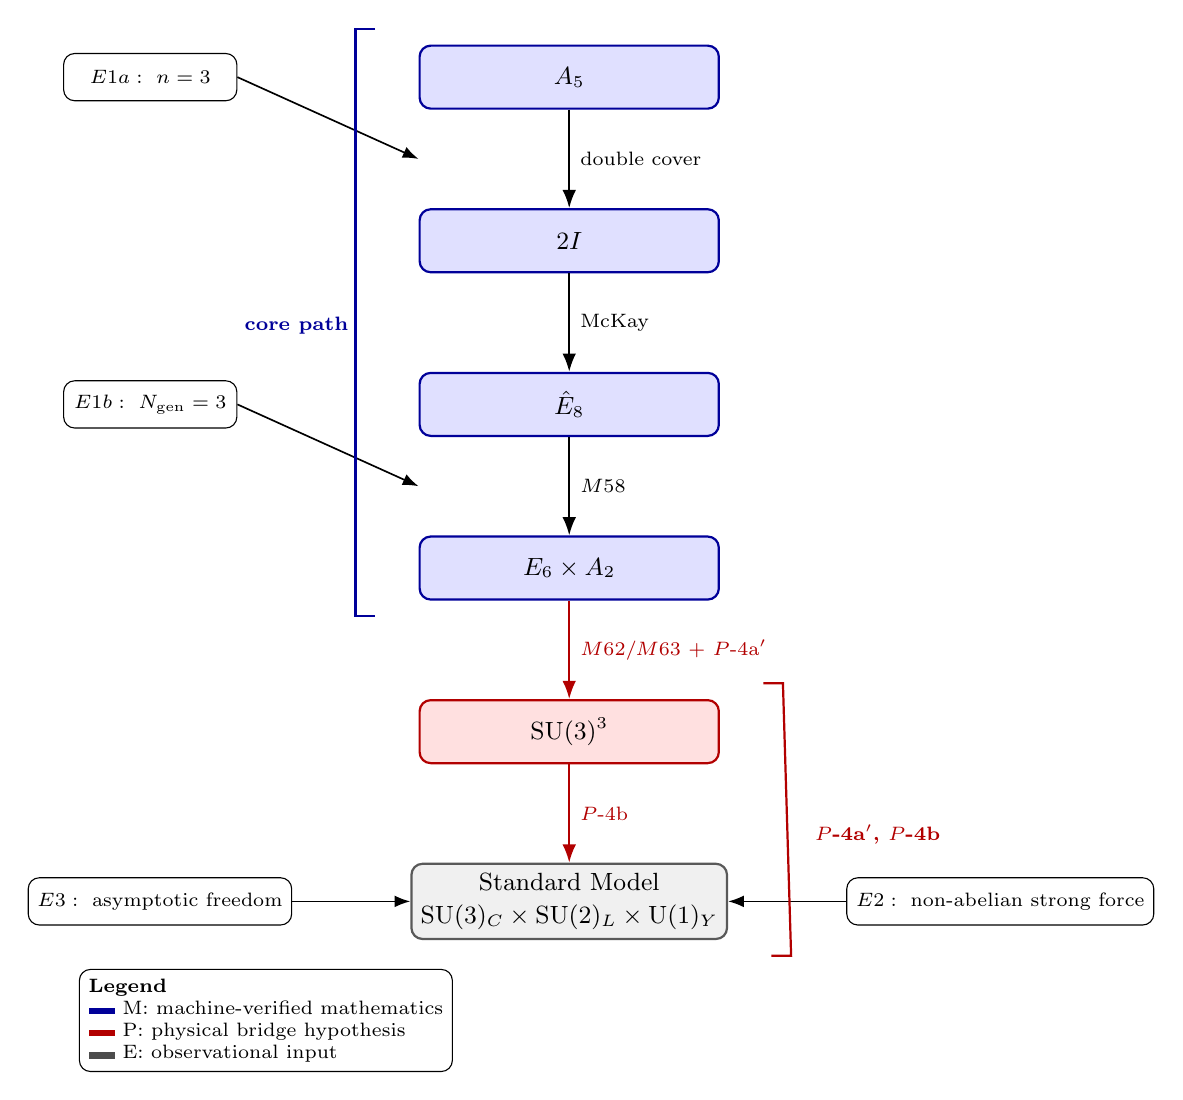
\begin{tikzpicture}[
  node distance=1.25cm and 2.7cm,
  >=Latex,
  font=\small,
  box/.style={draw, rounded corners, minimum width=3.8cm, minimum height=8mm, align=center, thick},
  mbox/.style={box, fill=blue!12, draw=blue!60!black},
  pbox/.style={box, fill=red!12, draw=red!70!black},
  ebox/.style={box, fill=black!6, draw=black!65},
  aux/.style={draw, rounded corners, minimum width=2.2cm, minimum height=6mm, align=center, font=\scriptsize, fill=white},
  lab/.style={font=\scriptsize, inner sep=1pt, outer xsep=3pt, fill=white, text=black},
  noteM/.style={font=\scriptsize\bfseries, text=blue!60!black},
  noteP/.style={font=\scriptsize\bfseries, text=red!70!black},
  noteE/.style={font=\scriptsize\bfseries, text=black!80}
]

\node[mbox] (a5) {$A_5$};
\node[mbox, below=of a5] (twoi) {$2I$};
\node[mbox, below=of twoi] (e8) {$\Ehat_8$};
\node[mbox, below=of e8] (e6a2) {$E_6\times A_2$};
\node[pbox, below=of e6a2] (su333) {$\SU(3)^3$};
\node[ebox, below=of su333] (sm) {Standard Model\\[1pt]
$\SU(3)_C\times \SU(2)_L\times \U(1)_Y$};

\draw[->, thick] (a5) -- node[lab, right] {double cover} (twoi);
\draw[->, thick] (twoi) -- node[lab, right] {McKay} (e8);
\draw[->, thick] (e8) -- node[lab, right] {$M58$} (e6a2);
\draw[->, thick, red!70!black] (e6a2) -- node[lab, right, text=red!70!black] {$M62/M63$ + $P$-4a$'$} (su333);
\draw[->, thick, red!70!black] (su333) -- node[lab, right, text=red!70!black] {$P$-4b} (sm);

\node[aux, left=2.3cm of a5] (e1a) {$E1a:\ n=3$};
\node[aux, left=2.3cm of e8] (e1b) {$E1b:\ N_{\mathrm{gen}}=3$};
\node[aux, right=1.5cm of sm] (e2) {$E2:\ \text{non-abelian strong force}$};
\node[aux, left=1.5cm of sm] (e3) {$E3:\ \text{asymptotic freedom}$};

\draw[->, semithick] (e1a.east) -- ($(a5.west)!0.5!(twoi.west)$);
\draw[->, semithick] (e1b.east) -- ($(e8.west)!0.5!(e6a2.west)$);
\draw[->, semithick] (e2.west) -- (sm.east);
\draw[->, semithick] (e3.east) -- (sm.west);

\draw[blue!60!black, thick]
  ($(a5.north west)+(-0.55,0.2)$) -- ($(a5.north west)+(-0.8,0.2)$)
  -- ($(e6a2.south west)+(-0.8,-0.2)$) -- ($(e6a2.south west)+(-0.55,-0.2)$);
\node[noteM] at ($(e8.west)+(-1.55,1.0)$) {core path};

\draw[red!70!black, thick]
  ($(su333.north east)+(0.55,0.2)$) -- ($(su333.north east)+(0.8,0.2)$)
  -- ($(sm.south east)+(0.8,-0.2)$) -- ($(sm.south east)+(0.55,-0.2)$);
\node[noteP] at ($(sm.east)+(1.9,0.85)$) {$P$-4a$'$, $P$-4b};

\node[draw, rounded corners, fill=white, align=left, font=\scriptsize, anchor=north west]
      at ($(e3.south west)+(0.65,-0.55)$) {
\textbf{Legend}\\
\textcolor{blue!60!black}{\rule{1.2em}{0.8ex}}~M: machine-verified mathematics\\
\textcolor{red!70!black}{\rule{1.2em}{0.8ex}}~P: physical bridge hypothesis\\
\textcolor{black!70}{\rule{1.2em}{0.8ex}}~E: observational input
};

\end{tikzpicture}
\caption{Vertical overview of the pathway $A_5\to 2I\to \Ehat_8\to E_6\times A_2\to \SU(3)^3\to \mathrm{SM}$. The mathematically fixed core path is shown in blue, while the irreducible physical inputs are localized at $P$-4a$'$ and $P$-4b (red). External observational inputs are $E1a$, $E1b$, $E2$, and $E3$.}
\label{fig:vertical_pathway}
\end{figure}


The central problem of this paper is to identify what is mathematically fixed
at each stage of this pathway and what still requires physical judgment.  To
anticipate the conclusion, assuming the framework hypothesis $\mathrm{FA}_1$
(physical development of the McKay correspondence, \S\ref{sec:mckay}), the
core path $A_5 \to 2I \to \Ehat_8 \to E_6 \times A_2$ is uniquely fixed in
the M~layer with only two empirical inputs: $n = 3$ and $\Ngen = 3$.  On the
other hand, in the final stage $E_6 \to \SU(3)^3 \to \text{SM}$, two points
remain as irreducible physical inputs: the equal-rank democracy
requirement~P-4a$'$ and the color identification~P-4b.

The main findings of this paper can therefore be summarized as follows.

\paragraph{Main result~1 (rigidity).}
The route $A_5 \to 2I \to \Ehat_8 \to E_6 \times A_2$ is uniquely fixed in
the M~layer with $E_{1a}$~($n=3$) and $E_{1b}$~($\Ngen = 3$) as the sole
external inputs.  This is supported by M49 (McKay--family dictionary),
M50--M57 (CP structure), and M58--M61 ($E_8$ selection and node removal
classification).

\paragraph{Main result~2 (localization of physical arbitrariness).}
The structural degrees of freedom that remain in the P~layer throughout the
entire path are localized to two points, P-4a$'$ and P-4b.  In particular,
the candidate space for trinification itself is uniquely determined by finite
enumeration using M62/M63, but the physical reasons for its adoption and the
identification of its color remain outside of algebra.

In this sense, the argument of this paper is not the ``derivation of the
entire path to the Standard Model'' itself, but rather the precise
determination of ``to what extent mathematics determines the path to the
Standard Model, and from what point onward it belongs to physics.''


\subsection{Original contributions of this paper}\label{sec:contributions}

In addition to the two main results, the unique contribution of this paper is
the trinification stage ($E_6 \to \SU(3)^3$): decomposing the problem into
fixing the candidate space (M62/M63, \layerM) and the physical reason for
adoption (P-4a$'$, \layerP), and then condensing the content of~P.
Furthermore, through an audit of all 25 internal hypotheses, we show that
$\Amin$ can be reduced to 6 hypotheses (with only 2 structural~Ps).


\subsection{Structure of the paper}\label{sec:structure}

Section~\ref{sec:mckay-family} discusses the McKay correspondence and family
structure~(M49).  Section~\ref{sec:CP} discusses the CP
structure~(M50--M57).  Section~\ref{sec:E8selection} discusses the uniqueness
of $E_8 \to E_6 \times A_2$~(M58--M61).
Section~\ref{sec:trinification} discusses trinification selection and P4
three-stage decomposition~(M62--M63).
Section~\ref{sec:Sigmamin} discusses the minimal hypothesis set and its
epistemological significance.  Section~\ref{sec:comparison} discusses
comparisons with other theories and future prospects.
Section~\ref{sec:conclusion} presents the conclusions.  Appendix~\ref{app:lean}
contains the Lean~4 verification system, Appendix~\ref{app:gap} contains the
GAP verification scripts, and Appendix~\ref{app:Phypotheses} contains a
complete list of P-layer hypotheses.


%% ====================================================================
%%  §2. McKay Compatibility and Family Structure
%% ====================================================================
\section{McKay compatibility and family structure}\label{sec:mckay-family}

The purpose of this section is to describe the McKay correspondence from the
double covering group $2I$ of $A_5$ to the affine $\Ehat_8$ Dynkin diagram,
and to uniquely identify which irreducible representation of $A_5$ corresponds
to the ``3'' in $(27,3)$ within the $E_8 \to E_6 \times A_2$ branch.  All
content in this section belongs to the M~layer.


\subsection{The binary icosahedral group $2I$ and the McKay correspondence}\label{sec:mckay}

$A_5$ (alternating group, order~60) has five irreducible representations:
$\rho_1$~(trivial, dim~1), $\rho_3$~(dim~3), $\rho_3'$~(dim~3),
$\rho_4$~(dim~4), and $\rho_5$~(dim~5), satisfying $\sum d_i^2 = 1 + 9 + 9 +
16 + 25 = 60 = |A_5|$.  The pair $\rho_3$ and $\rho_3'$ are Galois
conjugates, distinguished by their character values on order-5 elements:
$\varphi = (1+\sqrt{5})/2$ and $-1/\varphi = (1-\sqrt{5})/2$, respectively.

The Schur multiplier $H^2(A_5, \U(1)) = \mathbb{Z}_2$ gives $A_5$ a unique
double covering group~$2I$ (the binary icosahedral group, order~120).  $2I$
inherits five representations of $A_5$ as ``$A_5$-type'' and additionally has
four ``spinorial'' representations $s_2$, $s_2'$, $s_4$, $s_6$ (dim~2, 2, 4,
6).  With a total of nine irreducible representations, $\sum d_i^2 = 120 =
|2I|$ holds.

The McKay correspondence (McKay 1980~\cite{McKay1980}; geometric formulation
by Gonzalez-Sprinberg--Verdier~\cite{GSV1983}) asserts that the graph (McKay
graph) defined by taking irreducible representations of a finite subgroup
$\Gamma \subset \SU(2)$ as vertices and the tensor product decomposition law
with the fundamental representation of $\SU(2)$ as edges coincides with the
corresponding affine Dynkin diagram.  For $2I$, the McKay graph coincides with
affine $\Ehat_8$~\layerM, which is a purely mathematical fact provable by
direct computation of representation theory.

\paragraph{Methodological note ($\mathrm{FA}_1$).}
The output of the McKay correspondence is an affine Dynkin diagram---a graph
isomorphic to the classification labels of finite Lie algebras---and not the
Lie algebra itself.  The correspondence from the Dynkin diagram to a
semisimple Lie algebra is unique by Serre's theorem (1966~\cite{Serre1966})
\layerM, and the classification of the $E_8$ maximal subalgebra (\S\ref{sec:E8selection}), the
branching rules of representations, and the Frobenius--Schur indicators used
in this paper are all mathematical consequences derived from the structure of
this Lie algebra~\layerM.

On the other hand, the step of interpreting the Dynkin diagram output by the
McKay correspondence as an algebra of \emph{physical} gauge symmetry involves
a judgment that goes beyond the mathematical correspondence.
This judgment is explicitly separated as a framework hypothesis with two
logically distinct components:

\begin{quote}
\textbf{$\mathrm{FA}_{1a}$ (Canonical lift):}
Once one seeks a canonical Lie-theoretic structure attached to the $A_5$
data, the McKay correspondence uniquely selects affine~$\Ehat_8$.

\textbf{$\mathrm{FA}_{1b}$ (Physical adoption):}
This Lie-theoretic structure is taken as a candidate organizing principle
for gauge physics.
\end{quote}

$\mathrm{FA}_{1a}$ is mathematically motivated: the McKay output is unique
and canonical, Serre's theorem lifts it to a unique Lie algebra, and no
choice is involved.  However, the decision to regard this mathematical
structure as \emph{physically significant} is not itself a mathematical
theorem.  $\mathrm{FA}_{1b}$ is the genuine framework commitment.
The present work studies the physical consequences of adopting this canonical
lift; it does not claim that nature must follow this route.

$\mathrm{FA}_1$ differs in nature from the individual bridge hypotheses listed
in $\Amin$.  While each hypothesis in $\Amin$ is localized to a specific step
within the pathway, $\mathrm{FA}_1$ is an explicitly exposed framework choice
for unfolding the entire pathway.
$\mathrm{FA}_1$ should not be read as a hidden dynamical postulate.
Its role is to specify which canonical Lie-theoretic structure attached to the
$A_5$ data is taken as the starting point of the physical analysis.
The purpose of this paper is not to prove $\mathrm{FA}_1$ itself, but to
determine, once $\mathrm{FA}_1$ is adopted, which parts of the pathway are
mathematically rigid and which remain genuinely physical.

\paragraph{Non-arbitrariness of $\mathrm{FA}_1$.}
The non-arbitrariness of $\mathrm{FA}_1$ is supported by three mutually
independent considerations.

\emph{(i) Upstream uniqueness of $A_5$.}\enspace
Paper~I~\cite{Paper1} establishes $A_5$ as the unique non-solvable finite
subgroup of $SO(3)$.
If $A_5$ already occupies a distinguished position upstream, it is natural to
examine the canonical Lie-theoretic object attached to it via the McKay
correspondence.

\emph{(ii) Geometric reappearance.}\enspace
Kronheimer's construction~\cite{Kronheimer1989} shows that the same ADE
package appears independently in the geometry of ALE spaces as
hyper-K\"ahler quotients.
This demonstrates that the McKay correspondence is not merely a
graph-theoretic coincidence but reflects a deeper geometric structure.

\emph{(iii) Historical precedent in string theory.}\enspace
$E_8$-based algebraic structures recur in orbifold and heterotic string
constructions~\cite{GrossHarveyMartinecRohm1985}.
This does not by itself prove $\mathrm{FA}_1$, but it shows that
$\mathrm{FA}_1$ is not an \emph{ad hoc} insertion made solely for the
present pathway.

\paragraph{Counterfactual status of $\mathrm{FA}_1$.}
Table~\ref{tab:FA1-counterfactual} clarifies the consequences of accepting or
rejecting $\mathrm{FA}_1$.

\begin{table}[htb]
\centering
\caption{Counterfactual status of $\mathrm{FA}_1$.}\label{tab:FA1-counterfactual}
\begin{tabular}{p{0.45\textwidth}p{0.45\textwidth}}
\toprule
\textbf{$\mathrm{FA}_1$ adopted} & \textbf{$\mathrm{FA}_1$ rejected} \\
\midrule
The McKay--$E_8$ route is read as a physically meaningful pathway. &
All M-layer theorems remain valid as pure mathematics; only their physical
interpretation is withdrawn. \\[4pt]
$E_6 \times A_2$ selection, trinification, and CP structure acquire physical
significance. &
The pathway $A_5 \to E_8 \to E_6 \times A_2 \to \SU(3)^3$ becomes a
mathematical curiosity without physical content. \\[4pt]
Experimentally testable consequences arise (\S\ref{sec:falsifiability}). &
No physics claims of this paper are operative. \\
\bottomrule
\end{tabular}
\end{table}

If $\mathrm{FA}_1$ is physically meaningful, it should be tested indirectly
through the specific pattern of $E_6 \times A_2$ selection (M58), the
trinification-based branching relations (\S\ref{sec:falsifiability}), and the
gauge-coupling unification window.
In particular, if the generation structure predicted by $\rho_3'$ (M49) is
systematically inconsistent with observed flavor data, or if the
gauge-coupling running is incompatible with the $E_8$ Coxeter structure, then
$\mathrm{FA}_1$ would be indirectly falsified.
Therefore, all conclusions in this paper should be read with the condition
``under $\mathrm{FA}_1$''.


\subsection{Node structure of $\Ehat_8$ and marks}\label{sec:marks}

The affine $\Ehat_8$ graph is a tree graph with 9~vertices and 8~edges, with
the following adjacency structure:
\begin{equation}\label{eq:E8graph}
  0 \text{---} 8 \text{---} 7 \text{---} 6 \text{---} 5 \text{---} 4
  \text{---} 3 \text{---} 1,
  \qquad
  4 \text{---} 2 \quad (\text{branch}).
\end{equation}
The mark ($= $ dimension $d_k$ of the corresponding $2I$ irreducible
representation) of each node~$k$ is given in Table~\ref{tab:marks}.

\begin{table}[htb]
\centering
\caption{Marks of the affine $\Ehat_8$ McKay graph nodes.}\label{tab:marks}
\begin{tabular}{l*{9}{c}}
\toprule
Node & 0 & 1 & 2 & 3 & 4 & 5 & 6 & 7 & 8 \\
\midrule
Mark & 1 & 2 & 3 & 4 & 6 & 5 & 4 & 3 & 2 \\
\bottomrule
\end{tabular}
\end{table}

The sum of marks equals the Coxeter number $h = 30$ for $E_8$~\layerM:
\begin{equation}\label{eq:mark-sum}
  \sum_{k=0}^{8} d_k = 1 + 2 + 3 + 4 + 6 + 5 + 4 + 3 + 2 = 30 = h_{E_8}.
\end{equation}

Node~4 is the unique trivalent (branch) vertex, with mark~$= 6$
corresponding to the maximum-dimensional spinorial representation $s_6$
of~$2I$.  The location of this bifurcation plays an essential role in the
parity classification and Galois pair structure described below.

\noindent\textit{Lean verification:}
\texttt{marks\_sum\_coxeter}, \texttt{branch\_point\_unique}
(E8BlowUp.lean).


\subsection{Parity classification}\label{sec:parity}

The fundamental node in the McKay graph (node~8, dim~2, the fundamental
representation of $\SU(2)$) corresponds to the half-integer spin
representation.  On the McKay graph, the nine nodes are separated into two
classes---$A_5$-type (integer spin) and spinorial (half-integer
spin)---depending on whether their distance from the fundamental node is even
or odd.  The affine node~0 is a trivial representation ($j = 0$) and belongs
to $A_5$-type.  This parity is completely determined by the topology of the
McKay graph~\layerM.

\begin{table}[htb]
\centering
\caption{Parity classification of $\Ehat_8$ nodes.}\label{tab:parity}
\begin{tabular}{llll}
\toprule
Type & Node set & Dimensions & $\sum d_i^2$ \\
\midrule
$A_5$-type & $\{0,2,3,5,7\}$ & $\{1,3,4,5,3\}$ & 60 $(= |A_5|)$ \\
Spinorial  & $\{1,4,6,8\}$   & $\{2,6,4,2\}$   & 60 \\
\bottomrule
\end{tabular}
\end{table}

The equality $\sum d_i^2 = 60$ for both types reflects that the $A_5$-type
representations correspond exactly to all representations of $A_5$, and that
$|A_5| = |2I|/2 = 60$.

All five $A_5$-type representations have Frobenius--Schur indicator $\nu_2 =
+1$ (real type), and all four spinorial representations have $\nu_2 = -1$
(quaternionic type)~\layerM.  This fact provides the starting point for the CP
structure in~\S\ref{sec:CP}.

\noindent\textit{Lean verification:}
\texttt{A5type\_marks\_sq\_sum}, \texttt{spinorial\_marks\_sq\_sum}
(A5CP.lean).


\subsection{Galois pair $\{$node~2, node~7$\}$ = $\{\rho_3, \rho_3'\}$}\label{sec:galois-pair}

Among the $A_5$-type nodes, the only nodes with dim~$= 3$ are $\{2, 7\}$~%
\layerM.  Since there are only two dim-3 irreducible representations of
$A_5$, $\rho_3$ and $\rho_3'$, the set correspondence
$\{\text{node~2, node~7}\} = \{\rho_3, \rho_3'\}$ is uniquely determined.

Node~2 connects directly to the branch point (node~4) and corresponds to the
restriction of the $j = 1$ representation of $\SU(2)$ to~$2I$.  This is a
natural 3-dimensional action as an icosahedral rotation of $A_5 \subset \SO(3)$
and identifies with the representation $\rho_3$ where the character value on
the order-5 element is $\varphi = (1+\sqrt{5})/2$.  Node~7 is the remaining
dim-3 $A_5$-type node and identifies with $\rho_3'$ where the character value
on the order-5 element is $-1/\varphi = (1-\sqrt{5})/2$.  The pair $\rho_3$
and $\rho_3'$ are exchanged by the Galois automorphism $\sigma\colon
\sqrt{5}\mapsto -\sqrt{5}$ (M29~\cite{Paper1}; the complete structure of
$\sigma$ is formulated in \S\ref{sec:M54}).

\noindent\textit{Lean verification:}
\texttt{M49\_dim3\_A5type}, \texttt{mckayNode\_injective} (A5CP.lean),
\texttt{M29\_galois\_permutes\_chars} (FlavorGalois.lean).


\subsection{M49: McKay--family dictionary}\label{sec:M49}

According to M58 (detailed in \S\ref{sec:M58}), $E_6 \times A_2$ is uniquely
selected as the maximal subalgebra of $E_8$.  In the branch from $E_8$ to
$E_6 \times A_2$, the 248-dimensional adjoint representation is decomposed as:
\begin{equation}\label{eq:248branch}
  248 = (78,1) \oplus (1,8) \oplus (27,3) \oplus (\overline{27},\bar{3}).
\end{equation}
Here the ``3'' in $(27,3)$ is $\mathrm{fund}(A_2) =
\mathrm{fund}(\SU(3)_{\mathrm{family}})$, the carrier of the family index
and the algebraic origin of the 3-generation structure.  The purpose of M49 is
to identify which irreducible representation of $A_5$ corresponds to this~``3.''

In McKay-compatible language, $E_8 \to E_6 \times A_2$ corresponds to the
operation of removing node~7 from affine $\Ehat_8$ (M47, M60~\layerM).  The
mark of the removed node~7 is~3, and the residual Dynkin diagram decomposes
into $E_6 + A_2$ (M59~\layerM).

From this structure, the ``3'' of $(27,3)$ is determined by the chain:
mark of node~7 $\to$ parity classification $\to$ dim-3 $A_5$-type uniqueness
$\to$ $\rho_3'$ identification.  Each step is closed at~\layerM, and there is
no room for choice.  Note that the number of fermion generations~$= 3$
\layerE\ ($= E_{1b}$) is referenced as the C3 condition of M58
(\S\ref{sec:M58}).


\begin{figure}[t]
\centering
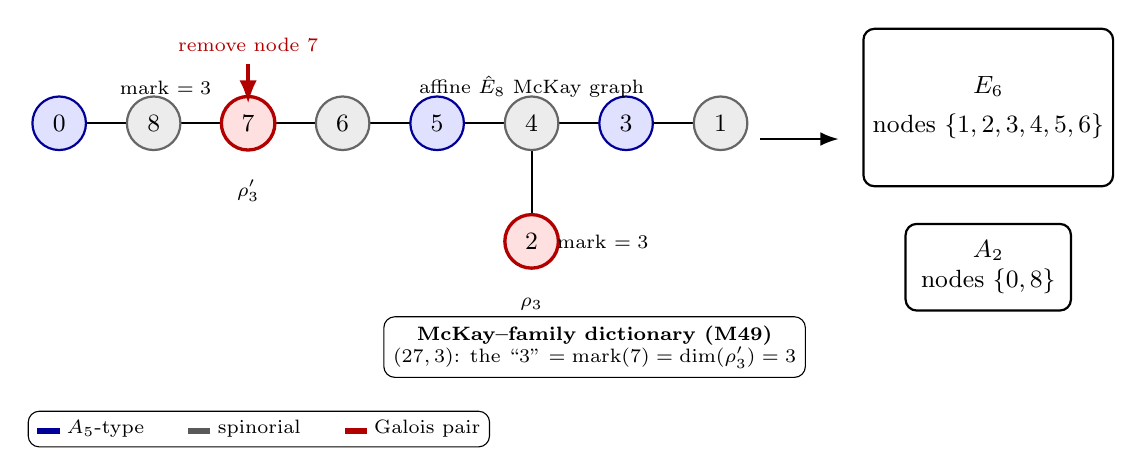
\begin{tikzpicture}[
  >=Latex,
  font=\small,
  nodebox/.style={circle, draw, minimum size=6.8mm, inner sep=0pt, thick},
  a5node/.style={nodebox, fill=blue!12, draw=blue!60!black},
  spinode/.style={nodebox, fill=gray!15, draw=black!60},
  hi/.style={nodebox, fill=red!12, draw=red!70!black, very thick},
  txt/.style={font=\scriptsize},
  smallbox/.style={draw, rounded corners, minimum width=2.2cm, minimum height=7mm, align=center, thick}
]

% left: original graph
\coordinate (n0) at (0,0);
\coordinate (n8) at (1.2,0);
\coordinate (n7) at (2.4,0);
\coordinate (n6) at (3.6,0);
\coordinate (n5) at (4.8,0);
\coordinate (n4) at (6.0,0);
\coordinate (n3) at (7.2,0);
\coordinate (n1) at (8.4,0);
\coordinate (n2) at (6.0,-1.5);

\draw[thick] (n0)--(n8)--(n7)--(n6)--(n5)--(n4)--(n3)--(n1);
\draw[thick] (n4)--(n2);

\node[a5node] at (n0) {0};
\node[spinode] at (n8) {8};
\node[hi] at (n7) {7};
\node[spinode] at (n6) {6};
\node[a5node] at (n5) {5};
\node[spinode] at (n4) {4};
\node[a5node] at (n3) {3};
\node[spinode] at (n1) {1};
\node[hi] at (n2) {2};

\node[txt, above=2mm of $(n4)$] {affine $\Ehat_8$ McKay graph};
\node[txt, below=6mm of n7] {$\rho_3'$};
\node[txt, below=6mm of n2] {$\rho_3$};
\node[txt] at (1.35,0.45) {mark $=3$};
\node[txt, right=2mm of n2] {mark $=3$};

\draw[->, very thick, red!70!black] (2.4,0.75) -- (2.4,0.25);
\node[txt, red!70!black] at (2.4,1.0) {remove node 7};

% right: residual decomposition
\node[smallbox, minimum width=2.6cm, minimum height=2.0cm, anchor=west] (e6box) at (10.2,0.2) {$E_6$\\[1mm]nodes $\{1,2,3,4,5,6\}$};
\node[smallbox, minimum width=2.1cm, minimum height=1.1cm, below=0.45cm of e6box] (a2box) {$A_2$\\nodes $\{0,8\}$};
\draw[->, thick] (8.9,-0.2) -- (9.9,-0.2);

\node[draw, rounded corners, fill=white, align=center, font=\scriptsize, anchor=north] at (6.8,-2.45)
{\textbf{McKay--family dictionary (M49)}\\
$(27,3)$: the ``3'' $= \mathrm{mark}(7)=\dim(\rho_3')=3$};

\node[draw, rounded corners, fill=white, font=\scriptsize, anchor=north west] at (-0.4,-3.65)
{\textcolor{blue!60!black}{\rule{1.0em}{0.7ex}}~$A_5$-type\qquad
\textcolor{black!65}{\rule{1.0em}{0.7ex}}~spinorial\qquad
\textcolor{red!70!black}{\rule{1.0em}{0.7ex}}~Galois pair};

\end{tikzpicture}
\caption{McKay--family dictionary. The two dim-3 $A_5$-type nodes form the Galois pair $\{\rho_3,\rho_3'\} = \{$node~2, node~7$\}$. Removing node~7 yields $E_6 + A_2$, and the ``3'' in $(27,3)$ is uniquely identified with $\rho_3'$.}
\label{fig:mckay_family_dictionary}
\end{figure}

\begin{theorem}[M49: McKay--family dictionary]\label{thm:M49}
\begin{enumerate}
  \item[\textup{(a)}] By parity classification, the $A_5$-type nodes are
    $\{0,2,3,5,7\}$, and $\sum d_i^2 = 60 = |A_5|$ holds.
  \item[\textup{(b)}] The only $A_5$-type nodes with $\dim = 3$ are
    $\{2,7\}$, forming the Galois pair $\{\rho_3, \rho_3'\}$.
  \item[\textup{(c)}] Removing node~7 gives $E_6 \times A_2$, and
    $\mathrm{mark}(7) = 3 = \dim(\rho_3') = $ family dimension.
  \item[\textup{(d)}] The ``3'' in $(27,3)$ is uniquely identified as
    $\rho_3'$ of $A_5$.
\end{enumerate}
\end{theorem}

\noindent\textit{Lean verification:}
\texttt{mckayNode}, \texttt{M49\_node7\_is\_rho3p} (A5CP.lean).


\subsection{Galois pair splitting and dictionary rigidity}\label{sec:galois-splitting}

As a structural consequence of M49, the Galois pair $\{\rho_3, \rho_3'\}$
splits asymmetrically via the $E_8 \to E_6 \times A_2$ bifurcation.  $\rho_3$
(node~2) remains inside $E_6$ and participates in the gauge structure, while
$\rho_3'$ (node~7) is removed and becomes the family index.  This asymmetry
follows deterministically from the topology of the McKay graph and gives the
algebraic origin of the CP structure discussed in~\S\ref{sec:CP}
(M53--M57).

There is no alternative-by-convention for the M49 identification.  Each step
of Theorem~\ref{thm:M49}\,(a)--(d) is uniquely determined in the M~layer.
The only convention dependence is ``how to label $\rho_3$ versus $\rho_3'$'',
and the structure as a Galois pair is convention-independent.


%% ====================================================================
%%  §3. CP Structure: From A₅ to E₆
%% ====================================================================
\section{CP structure: from $A_5$ to $E_6$}\label{sec:CP}

The purpose of this section is to fully describe the algebraic structure of CP
violation in the M~layer.  To anticipate the conclusion, CP violation is
fundamentally impossible inside $A_5$~(M50), CP enters only as the phase
$\arg(\lambda_3)$ of the sole cubic invariant of $E_6$~(M52), and this
structure is uniquely realized as a Galois involution on the McKay
graph~(M53--M57).  Everything in this section belongs to the M~layer, provided
the $E_6 \times A_5$ framework is assumed.



\begin{figure}[t]
\centering
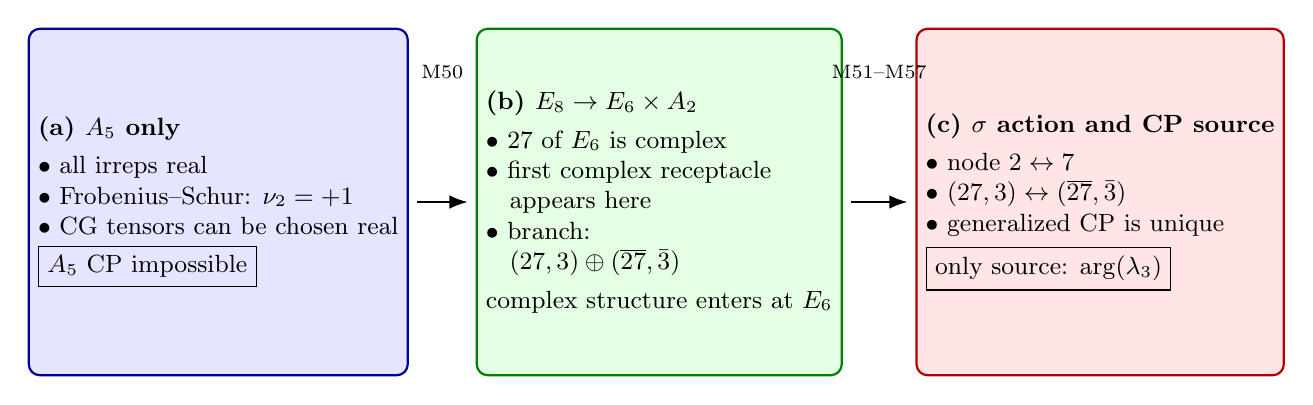
\begin{tikzpicture}[
  >=Latex,
  font=\small,
  panel/.style={draw, rounded corners, minimum width=3.5cm, minimum height=4.4cm, align=left, thick},
  title/.style={font=\small\bfseries},
  emph/.style={font=\scriptsize\bfseries}
]

\node[panel, fill=blue!10, draw=blue!60!black] (p1) at (0,0)
{\textbf{(a) $A_5$ only}\\[1mm]
$\bullet$ all irreps real\\
$\bullet$ Frobenius--Schur: $\nu_2=+1$\\
$\bullet$ CG tensors can be chosen real\\[1mm]
\centering\fbox{$A_5$ CP impossible}
};

\node[panel, fill=green!10!white, draw=green!50!black] (p2) at (5.6,0)
{\textbf{(b) $E_8\to E_6\times A_2$}\\[1mm]
$\bullet$ $27$ of $E_6$ is complex\\
$\bullet$ first complex receptacle\\
\hspace*{3mm}appears here\\
$\bullet$ branch:\\
\hspace*{3mm}$(27,3)\oplus (\overline{27},\bar 3)$\\[1mm]
\centering complex structure enters at $E_6$
};

\node[panel, fill=red!10, draw=red!70!black] (p3) at (11.2,0)
{\textbf{(c) $\sigma$ action and CP source}\\[1mm]
$\bullet$ node $2\leftrightarrow 7$\\
$\bullet$ $(27,3)\leftrightarrow (\overline{27},\bar 3)$\\
$\bullet$ generalized CP is unique\\[1mm]
\centering\fbox{only source: $\arg(\lambda_3)$}
};

\draw[->, thick] ($(p1.east)+(0.1,0)$) -- ($(p2.west)+(-0.1,0)$);
\draw[->, thick] ($(p2.east)+(0.1,0)$) -- ($(p3.west)+(-0.1,0)$);

\node[font=\scriptsize, align=center] at ($(p1.east)!0.5!(p2.west)+(0,1.65)$) {M50};
\node[font=\scriptsize, align=center] at ($(p2.east)!0.5!(p3.west)+(0,1.65)$) {M51--M57};

\end{tikzpicture}
\caption{Three-step summary of the CP structure. CP violation is impossible inside $A_5$ (M50), a complex receptacle first appears at the $E_8\to E_6\times A_2$ bifurcation (M51), and the generalized CP transformation is realized by the Galois involution $\sigma$, with unique CP source $\arg(\lambda_3)$ (M52--M57).}
\label{fig:cp_structure_summary}
\end{figure}

\subsection{M50: $A_5$ CP impossibility theorem}\label{sec:M50}

\begin{theorem}[M50]\label{thm:M50}
The five irreducible representations of $A_5$ --- $\rho_1$, $\rho_3$,
$\rho_3'$, $\rho_4$, $\rho_5$ --- are all of real type
(Frobenius--Schur indicator $\nu_2 = +1$).
\end{theorem}

The proof is direct.  The Frobenius--Schur indicator $\nu_2(\rho) = (1/|G|)
\sum_{g \in G} \chi_\rho(g^2)$ can be evaluated in finite computation as a sum
over the five conjugacy classes of $A_5$.  For all five representations, we
obtain $\nu_2 = +1$.

The condition $\nu_2 = +1$ means, by Frobenius' theorem, that the
representation admits a real basis.  From this, all representation matrices can
be taken real, and by Wigner's theorem (finite group version), the
Clebsch--Gordan coefficients can also be chosen real.  Therefore, all
couplings of $A_5$-invariant potentials are real, and all rephasing-invariant
CP phases vanish:
\begin{equation}\label{eq:A5CPimpossible}
  \fbox{$A_5$ CP violation is impossible with $A_5$ symmetry alone.}
\end{equation}

A complex structure outside of $A_5$ is essential to generate the CP phase.

\noindent\textit{Lean verification:}
\texttt{M50\_all\_real\_type} (A5CP.lean, \texttt{native\_decide}).
\textit{GAP verification:} \texttt{Indicator(CharacterTable("A5"), [chi], 2)}
(M50\_M54\_verify.gap).


\subsection{M51: $E_6$ fundamental $27$ is complex type}\label{sec:M51}

\begin{theorem}[M51]\label{thm:M51}
The fundamental representation~$27$ of $E_6$ is of complex type
$(27 \not\cong \overline{27})$.
\end{theorem}

The Dynkin diagram of $E_6$ has a non-trivial $\mathbb{Z}_2$ diagram
automorphism, which swaps node~$1 \leftrightarrow$ node~$6$.  This
automorphism induces the highest weight exchange $\omega_1 \leftrightarrow
\omega_6$.  Since $\omega_1 \neq \omega_6$, it follows that
$27 = V(\omega_1) \not\cong V(\omega_6) = \overline{27}$.

The comparison between M50 and M51 clarifies the algebraic origin of~CP:

\begin{table}[htb]
\centering
\caption{Comparison of $A_5$ and $E_6$ CP structures.}\label{tab:CP-compare}
\begin{tabular}{lll}
\toprule
 & $A_5$ & $E_6$ \\
\midrule
Fundamental rep.\ type & All real ($\nu_2 = +1$) & $27$ is complex \\
Dynkin diagram symmetry & Self-evident (all real) & $\mathbb{Z}_2$
  ($\omega_1 \leftrightarrow \omega_6$) \\
CP phase & Impossible & Allowed \\
\bottomrule
\end{tabular}
\end{table}

On the path from $A_5$ to $E_6$, the complex representation first appears at
the bifurcation point $E_8 \to E_6 \times A_2$---that is, the moment when
$(27,3)$ separates from~248.  The algebraic origin of the CP phase is
precisely localized at this bifurcation point.

\noindent\textit{Lean verification:}
\texttt{M51\_E6\_27\_isComplex}, \texttt{M51\_E6\_27\_ne\_27bar}
(E6Complex.lean, \texttt{decide}).


\subsection{M52: Uniqueness of CP source}\label{sec:M52}

\begin{theorem}[M52]\label{thm:M52}
In an $E_6 \times A_5$-invariant renormalizable theory (mass term + cubic +
quartic), the only independent CP-violating phase is $\arg(\lambda_3)$ of the
$27^3$ cubic coupling.
\end{theorem}

This theorem consists of four sub-results:

\textbf{M52a}~\layerM: $\dim \Inv(\Sym^3(27_{E_6})) = 1$.  That is, $E_6$
has exactly one cubic invariant $d_{ijk}$ on~27.  The proof begins with the
complete decomposition $27 \otimes 27 = V(2\omega_1) \oplus V(\omega_3) \oplus
\overline{27}$, where $V(2\omega_1) = \mathbf{351}$, $V(\omega_3) =
\mathbf{351}'$, and the dimension is consistent as $351 + 351 + 27 = 729 =
27^2$.  Since $\overline{27}$ belongs to $\Sym^2(27)$, the invariant belongs to
$\Sym^3(27)$, and its dimension is~1.

\textbf{M52b}~\layerM: From M50, the $A_5$-invariant CG tensor can be taken
with a real basis.

\textbf{M52c}~\layerM: The quartic coupling is real by hermiticity.  Since
$(27 \times \overline{27})^2$ is self-adjoint, the quartic coupling constant
can be taken real.

\textbf{M52d}~\layerM: Under the field rephasing $\Phi \to e^{i\alpha}\Phi$,
$\lambda_3 \to e^{3i\alpha}\lambda_3$, but $\arg(\lambda_3)$ cannot be
removed because it affects other couplings (mass term, quartic term).

Combining these four sub-results, the sole source of CP violation in the
$E_6 \times A_5$-invariant theory is localized to $\arg(\lambda_3)$:
\begin{equation}\label{eq:CPcondition}
  \delta_{\mathrm{CP}} = 0
  \;\Longleftrightarrow\;
  \arg(\lambda_3) = 0 \bmod \pi.
\end{equation}

The attribution of M52 is~\layerMs.  If we accept $E_6 \times A_5$ as a
framework, the uniqueness of the CP source is a purely mathematical
consequence, but the framework $E_6 \times A_5$ itself depends on M58 in
\S\ref{sec:E8selection}.

\emph{Scope of applicability.}
M52 holds within renormalizable theory (mass term $+$ cubic $+$ quartic).
The possibility of additional CP sources from effective operators of
$\dim \geq 5$ depends on the UV completion and is beyond the scope of this
paper.

\noindent\textit{Lean verification:} \texttt{M52\_unique\_CP\_source}
(A5CP.lean).  \textit{GAP verification:} M52a\_verify\_v2.gap.


\subsection{M54: Structure of Galois involution on the McKay graph}\label{sec:M54}

\begin{theorem}[M54]\label{thm:M54}
The Galois automorphism $\sigma\colon \sqrt{5} \mapsto -\sqrt{5}$ acts as an
involution on the 9 irreducible representations of $2I$.  $\sigma$ consists
of two transpositions:
\begin{equation}\label{eq:sigma-transpositions}
  \rho_3 \leftrightarrow \rho_3'
  \quad (A_5\text{-type}),
  \qquad
  s_2 \leftrightarrow s_2'
  \quad (\text{spinorial}),
\end{equation}
with five fixed points $\{\rho_1, \rho_4, \rho_5, s_4, s_6\}$.
\end{theorem}

$\sigma$ preserves dimension ($d_{\sigma(i)} = d_i$), parity ($A_5$-type
$\leftrightarrow$ $A_5$-type, spinorial $\leftrightarrow$ spinorial), and the
Frobenius--Schur indicator ($\nu_{2,\sigma(i)} = \nu_{2,i}$).

The $A_5$-type transposition $\rho_3 \leftrightarrow \rho_3'$ corresponds to
the exchange of node~$2 \leftrightarrow$ node~$7$ on the McKay graph.  The
fixed nodes $\rho_4$ (node~3) and $\rho_5$ (node~5) are $\sigma$-invariant
because they have rational character values.

The proof is carried out by implementing $\sigma$ as
$\mathrm{GaloisCyc}(\cdot, 2)$ in GAP---an automorphism that acts as
$\zeta_5 \mapsto \zeta_5^2$ over the cyclotomic field and induces
$\sqrt{5} \mapsto -\sqrt{5}$---and directly computing the action on the
character values of all 9 representations.

\noindent\textit{Lean verification:}
\texttt{M54\_involution}, \texttt{M54\_preserves\_dim},
\texttt{M54\_preserves\_parity}, \texttt{M54\_fixed\_count}
(A5CP.lean, \texttt{native\_decide}).


\subsection{M53, M55--M57: McKay--CP correspondence and channel
  splitting}\label{sec:M53-M57}

From M49 and M54, the following consequence theorems are derived.

\begin{theorem}[M53: McKay--CP correspondence]\label{thm:M53}
$\sigma$: node~$2 \leftrightarrow$ node~$7$ corresponds to the exchange
$(27,3) \leftrightarrow (\overline{27}, \bar{3})$ and gives the algebraic
framework of the generalized CP transformation.
\end{theorem}

This correspondence is a direct composition of M49 (node~$7 = \rho_3'
\to$ family) and M54 ($\sigma$ swaps nodes~2 and~7).  Combined with the fact
that removal of node~7 yields $E_6 \times A_2$ (M60, \S\ref{sec:M60}),
$\sigma$ naturally emerges as a mapping that swaps $(27,3)$ and
$(\overline{27}, \bar{3})$ on the $E_8 \to E_6 \times A_2$ branch.

\noindent\textit{Lean verification:}
\texttt{M53\_sigma\_swaps\_nodes\_2\_7} (A5CP.lean).

\begin{theorem}[M55: $\sigma$ action on the 248 branching]\label{thm:M55}
$\sigma$ acts on the 248 branches of $E_8 \to E_6 \times \SU(3)$ as shown in
Table~\ref{tab:sigma248}.
\end{theorem}

\begin{table}[htb]
\centering
\caption{$\sigma$ action on 248 branch components.}\label{tab:sigma248}
\begin{tabular}{lll}
\toprule
Component & $\sigma$ action & Reason \\
\midrule
$(78,1)$ adjoint & fixed & adjoint is real type \\
$(1,8)$ adjoint  & fixed & $\SU(3)$ adjoint is real type \\
$(27,3)$  & $\to (\overline{27}, \bar{3})$ & M54: $\rho_3' \leftrightarrow \rho_3$ + M51 \\
$(\overline{27}, \bar{3})$ & $\to (27,3)$ & converse \\
\bottomrule
\end{tabular}
\end{table}

In $248 = 78 + 8 + 81 + 81$, $\sigma$ fixes the adjoint components
(86~dimensions) and exchanges the matter components (162~dimensions) as a
complex conjugate pair.

\noindent\textit{Lean verification:}
\texttt{M55\_involution\_248}, \texttt{M55\_swaps\_27} (A5CP.lean).

\begin{theorem}[M56: $\sigma$--CP uniqueness]\label{thm:M56}
$\Gal(\mathbb{Q}(\sqrt{5})/\mathbb{Q}) = \{\mathrm{id}, \sigma\}$ is a group
of order~2, and its only nontrivial Galois automorphism is~$\sigma$.  Thus,
the algebraic structure of the generalized CP transformation is uniquely
determined.
\end{theorem}

The CP conservation condition is equivalent to all couplings in the potential
being $\sigma$-invariant (belonging to~$\mathbb{Q}$).  Combined with M52, CP
violation is equivalent to $\arg(\lambda_3) \neq 0 \bmod \pi$.

\noindent\textit{Lean verification:}
\texttt{M56\_unique\_sigma} (A5CP.lean).

\begin{theorem}[M57: CP-sensitive channel splitting]\label{thm:M57}
$\sigma$ swaps $\rho_3$ and $\rho_3'$ while fixing $\rho_4$ and $\rho_5$.
Due to this asymmetry, the three flavor channels of $A_5$ behave essentially
differently in their sensitivity to CP.
\end{theorem}

The comparison is summarized in Table~\ref{tab:CPchannels}.

\begin{table}[htb]
\centering
\caption{CP sensitivity channel splitting.}\label{tab:CPchannels}
\begin{tabular}{lll}
\toprule
 & Channel~II (mass) & Channel~III (mixing) \\
\midrule
Tensor product & $\rho_3 \otimes \rho_3' \otimes \rho_5$ &
  $\rho_3 \otimes \rho_3' \otimes \rho_4$ \\
CG eigenvalue field & $\mathbb{Q}(\sqrt{5})$ & $\mathbb{Q}$ \\
CP character & CP-sensitive & CP-even \\
\bottomrule
\end{tabular}
\end{table}

In both channels, $\sigma$ exchanges $\rho_3 \leftrightarrow \rho_3'$, but the
key to the splitting lies in the third factor.  Since all character values of
$\rho_4$ are rational, the CG eigenvalues of Channel~III remain in
$\mathbb{Q}$ and are $\sigma$-invariant (CP-even), while in Channel~II, which
involves $\rho_5$, the Galois asymmetry propagates to the CG coefficients, and
the eigenvalues belong to $\mathbb{Q}(\sqrt{5})$ (CP-sensitive).

The CP phase $\delta_{\mathrm{CP}}$ arises from the interference of these two
channels, and its unique source is $\arg(\lambda_3)$~(M52).  The value of
$\delta_{\mathrm{CP}}$ itself depends on the VEV dynamics and belongs
to~\layerP, but the uniqueness of the location where CP can enter is closed in
layer~M.

\noindent\textit{Lean verification:}
\texttt{M57\_both\_sigma\_fixed} (A5CP.lean).


\subsection{Dependency structure between theorems}\label{sec:CP-dependency}

The eight theorems in this section converge from three independent logical
sequences.

\emph{Sequence~1 (CP impossibility):}
M50 $\to$ M52b $\to$ M52.  From the fact that all representations of $A_5$
are real type~(M50), the reality of CG tensors follows~(M52b), leading to the
uniqueness of the CP source~(M52).

\emph{Sequence~2 (CP admissibility):}
M51 $\to$ M52a $\to$ M52.  The complex type of $27$ in $E_6$~(M51) and the
uniqueness of cubic invariants~(M52a) converge to support~M52.

\emph{Sequence~3 (McKay--CP structure):}
M49 (\S\ref{sec:M49}) $\to$ M54 $\to$ M53, M55, M56, M57.  From the
synthesis of the McKay--family dictionary~(M49) and Galois involution~(M54),
the McKay--CP correspondence~(M53), the action on 248~(M55), uniqueness~(M56),
and channel splitting~(M57) are derived.

The three sequences merge at M52 and M57, establishing a complete CP structure
where ``the only source of CP is $\arg(\lambda_3)$'' and ``mass is
CP-sensitive and the mixing angle is CP-even.''


%% ====================================================================
%%  §4. Uniqueness of E₈ → E₆ × A₂
%% ====================================================================
\section{Uniqueness of $E_8 \to E_6 \times A_2$}\label{sec:E8selection}

In this section, we show that the branch from $E_8$ to $E_6 \times A_2$ is
unique under three conditions: product structure~(C1), complex type
representation~(C2), and family dimension~3~(C3) (M58).  Furthermore, we
re-derive the same conclusion from an alternative path of node removal in
affine $\Ehat_8$~(M59--M61), confirming that the two paths converge to the
same structure.


\subsection{M58: Maximal subalgebra selection theorem}\label{sec:M58}

The maximal subalgebras of $E_8$ have been fully classified by
Dynkin~(1957~\cite{Dynkin1957}).  There are a total of eight types: five
regular and three special; see Table~\ref{tab:E8max}.

\begin{table}[htb]
\centering
\caption{Maximal subalgebras of $E_8$.}\label{tab:E8max}
\begin{tabular}{clllr}
\toprule
\# & Candidate $H$ & Type & 248 branching & $\dim(\adj)$ \\
\midrule
1 & $D_8 = \SO(16)$ & regular & $120 + 128_s$ & 120 \\
2 & $A_8 = \SU(9)$ & regular & $80 + 84 + \overline{84}$ & 80 \\
3 & $A_4 \times A_4 = \SU(5)^2$ & regular & $\adj^2 + (5,10) + \text{c.c.}$ & 48 \\
4 & $E_6 \times A_2$ & regular & $78 + 8 + (27,3) + \text{c.c.}$ & 86 \\
5 & $E_7 \times A_1$ & regular & $133 + 3 + (56,2)$ & 136 \\
6 & $G_2 \times F_4$ & special & $14 + 52 + (7,26)$ & 66 \\
7 & $A_1$ (special) & special & --- & 3 \\
8 & $B_2$ (special) & special & --- & 10 \\
\bottomrule
\end{tabular}
\end{table}

The three selection criteria used in this paper are as follows.

\paragraph{C1 (product structure).}
$H$ is the product of at least two simple factors.  The condition is
determined by algebraic fact~\layerM, but the motivation for requiring a
product structure---the separation of gauge and family structures---involves a
physical judgment [P-leaning].  However, the bottom-up path in
\S\ref{sec:M59} (M59--M61) reaches the same conclusion independently of C1,
so when the two paths are combined, the P-like element of C1 is absorbed.  C1
eliminates four candidates: $D_8$, $A_8$, $A_1$(special), and $B_2$(special).

\paragraph{C2 (complex type representation).}
The branch of 248 to $H$ contains a complex component ($R \not\cong \bar{R}$).
The condition is determined by computing the Frobenius--Schur indicator~\layerM;
the motivation for requiring this is the existence of a CP phase
receptacle~(\S\ref{sec:M51}), which references the observational fact that CP
violation is physically realized~\layerE.  C2 further eliminates $E_7 \times
A_1$ and $G_2 \times F_4$.

The exclusion of $E_7 \times A_1$ merits careful consideration.  The
representation $\mathbf{56}$ of $E_7$ is pseudo-real ($\nu_2 = -1$), not complex.
$(56,2)$ lacks compatibility with the Yukawa coupling requiring a $\Sym^3$
structure and is also incompatible with C3 because its family dimension is~2.
$G_2 \times F_4$ is excluded because neither $G_2$ nor $F_4$ has non-trivial
Dynkin diagram automorphisms, so all representations are real type.

\paragraph{C3 (family dimension)~\layerE.}
The dimension of the fundamental representation of one of the factors is~3.
This is a reference to the observed fact of 3~generations~\layerE.  C3
eliminates $A_4 \times A_4$ (family dimension~$= 5$).

The results of applying the three conditions are summarized in
Table~\ref{tab:C123}.

\begin{table}[htb]
\centering
\caption{Application of selection criteria C1--C3.}\label{tab:C123}
\begin{tabular}{lcccc}
\toprule
Candidate & C1 & C2 & C3 & Result \\
\midrule
$D_8$ & $\times$ & --- & --- & excluded \\
$A_8$ & $\times$ & --- & --- & excluded \\
$A_4 \times A_4$ & $\checkmark$ & $\checkmark$ & $\times$ (5) & excluded \\
$E_6 \times A_2$ & $\checkmark$ & $\checkmark$ & $\checkmark$ (3) & \textbf{survives} \\
$E_7 \times A_1$ & $\checkmark$ & $\times$ & $\times$ (2) & excluded \\
$G_2 \times F_4$ & $\checkmark$ & $\times$ & --- & excluded \\
$A_1$ (special) & $\times$ & --- & --- & excluded \\
$B_2$ (special) & $\times$ & --- & --- & excluded \\
\bottomrule
\end{tabular}
\end{table}

\begin{theorem}[M58: Selection of $E_8$ maximal subalgebras]\label{thm:M58}
Of the 8 maximal subalgebras of $E_8$, only $E_6 \times A_2$ satisfies C1
(product structure) $\wedge$ C2 (complex type) $\wedge$ C3 (family
dimension~$= 3$) simultaneously.
\end{theorem}

The attribution of M58 is~\layerMs.  The determination of each condition is
algebraically decidable~\layerM.  The layer attribution of the motivations
for the conditions is: C1 is [P-leaning] (absorbable in M59--M61), C2 is
\layerE\ (existence of CP violation), and C3 is \layerE\ (3 generations).
Thus, M58 is a conditional M-layer theorem with \layerE\ as external input.

\noindent\textit{Lean verification:}
\texttt{M58\_E6A2\_unique\_selection}, \texttt{M58\_iff} (E8MaxSub.lean).


\subsection{M59: Complete classification of $\Ehat_8$ single-node removal}\label{sec:M59}

M58 was a top-down selection from the algebraic structure of the maximal
subalgebras of $E_8$.  In this section, we arrive at the same conclusion
through a bottom-up path of node removal in the affine $\Ehat_8$ McKay graph.

\begin{theorem}[M59]\label{thm:M59}
When node~$k$ ($k = 0, \ldots, 8$) is removed from affine $\Ehat_8$, the
remaining Dynkin type is as given in Table~\ref{tab:M59}.
\end{theorem}

\begin{table}[htb]
\centering
\caption{Complete classification of $\Ehat_8$ single-node removal.}\label{tab:M59}
\begin{tabular}{cclll}
\toprule
Node & Mark & $2I$ irrep & Residual Dynkin type & Lie group \\
\midrule
0 & 1 & $\rho_1$ (affine) & $E_8$ & $E_8$ \\
1 & 2 & spinorial & $D_8$ & $\SO(16)$ \\
2 & 3 & $\rho_3$ & $A_8$ & $\SU(9)$ \\
3 & 4 & $\rho_4$ & $A_1 + A_7$ & $\SU(2) \times \SU(8)$ \\
4 & 6 & spinorial & $A_1 + A_2 + A_5$ & $\SU(2) \times \SU(3) \times \SU(6)$ \\
5 & 5 & $\rho_5$ & $A_4 + A_4$ & $\SU(5)^2$ \\
6 & 4 & spinorial & $A_3 + D_5$ & $\SU(4) \times \SO(10)$ \\
7 & 3 & $\rho_3'$ & $E_6 + A_2$ & $E_6 \times \SU(3)$ \\
8 & 2 & spinorial & $A_1 + E_7$ & $\SU(2) \times E_7$ \\
\bottomrule
\end{tabular}
\end{table}

The proof is performed by finite enumeration (9 possibilities).  The connected
components of the remaining subgraphs after removing each node are determined,
and the Dynkin type is identified by arm-length analysis.  In all 9 cases, the
total rank of the residual type is $8 = \rank(E_8)$.

In Table~\ref{tab:M59}, removal of node~0 is the affine node removal,
recovering finite type $E_8$.  Only removal of node~4 (branch point, mark~$= 6$)
results in a 3-component residual.

\noindent\textit{Lean verification:}
\texttt{nodeRemovalResult}, \texttt{M59\_rank\_check},
\texttt{three\_components\_unique} (E8BlowUp.lean, \texttt{decide}).


\subsection{M60: Uniqueness of $E_6$ factor}\label{sec:M60}

\begin{theorem}[M60]\label{thm:M60}
Of the nine possibilities in M59, only removal of node~7 results in a residual
Dynkin type containing an $E_6$ factor.
\end{theorem}

This is verified by scanning Table~\ref{tab:M59}.

\noindent\textit{Lean verification:}
\texttt{M60\_E6\_factor\_unique} (E8BlowUp.lean, \texttt{decide}).


\subsection{M61: Mark-3 dichotomy}\label{sec:M61}

\begin{theorem}[M61: Mark-3 dichotomy]\label{thm:M61}
In $\Ehat_8$, the only nodes with $\mathrm{mark} = 3$ are $\{2, 7\}$.  Both
are $A_5$-type (\S\ref{sec:parity}) and correspond to the Galois pair
$\{\rho_3, \rho_3'\}$ (\S\ref{sec:galois-pair}).  However, the removal
results are fundamentally different:
\begin{center}
\begin{tabular}{lllcc}
\toprule
Node & $A_5$ irrep & Removal result & Product? & $E_6$ factor? \\
\midrule
7 & $\rho_3'$ & $E_6 + A_2$ & $\checkmark$ & $\checkmark$ \\
2 & $\rho_3$  & $A_8$        & $\times$     & $\times$ \\
\bottomrule
\end{tabular}
\end{center}
\end{theorem}

Removing node~7 yields $E_6 \times A_2$, opening a path to trinification.
Removing node~2 yields $A_8 = \SU(9)$ (single factor), making gauge/family
separation impossible.

In the Galois pair, the asymmetry whereby $\rho_3'$ (node~7) carries the
family index and $\rho_3$ (node~2) remains inside $E_6$ follows
deterministically from the topology of the McKay graph.  Node~7 is on the side
of the main chain closer to the affine node~0 (connected via node~8), while
node~2 is directly connected to the branch point (node~4).  This difference
fundamentally alters the connectivity structure of the graph after removal.

M61 can be restated as follows: the only node removal that simultaneously
satisfies ``$E_6$ factor $\wedge$ $A_2$ factor $\wedge$ mark~$= 3$'' is
node~7.  This is a node-removal version of M58 (C1 + C2 + C3).

\noindent\textit{Lean verification:}
\texttt{M61\_mark3\_dichotomy}, \texttt{galois\_pair\_asymmetry},
\texttt{galois\_separation} (E8BlowUp.lean, \texttt{decide}).


\subsection{Convergence of dual paths}\label{sec:convergence}

The theorem system in this section establishes the uniqueness of $E_8 \to E_6
\times A_2$ through two independent paths: top-down (M58: Dynkin
classification + C1/C2/C3 selection) and bottom-up (M59--M61: complete
enumeration of McKay graph nodes).  The triple fixation, combining these with
M49 (parity classification + Galois pairs), is summarized in
Table~\ref{tab:triple}.

\begin{table}[htb]
\centering
\caption{Triple convergence of independent paths.}\label{tab:triple}
\begin{tabular}{llll}
\toprule
Route & Starting point & Method & Conclusion \\
\midrule
M49 & McKay parity + Galois pair & Character analysis & $(27,3)$:
  $3 = \rho_3'$ \\
M58 & Dynkin maximal sub-classification & C1+C2+C3 & $E_6 \times A_2$ unique \\
M59--M61 & $\Ehat_8$ node removal & Complete enumeration & Node~7 unique \\
\bottomrule
\end{tabular}
\end{table}

The fact that three routes converge to the same structure from different
starting points and proof methods supports the structural necessity of $E_6
\times A_2$.


\subsection{$E_6$ internal node removal and connection to trinification}\label{sec:E6internal}

Sections~\ref{sec:M58}--\ref{sec:convergence} established the uniqueness of
$E_8 \to E_6 \times A_2$.  Before discussing $E_6 \to \SU(3)^3$ in
\S\ref{sec:trinification}, we analyze node removal within $E_6$ to confirm
why trinification cannot be achieved by simple Dynkin diagram operations.

The Dynkin diagram of $E_6$ has the structure:
\begin{equation}\label{eq:E6graph}
  6 \text{---} 5 \text{---} 4 \text{---} 3 \text{---} 1,
  \qquad
  4 \text{---} 2 \quad (\text{branch}).
\end{equation}

Removing the branch point (node~4, mark~$= 6$) yields $A_2 + A_2 + A_1 =
\SU(3) \times \SU(3) \times \SU(2)$, which is the node removal within $E_6$
that generates the most factors.  However, this does not reach the
trinification $\SU(3)^3$.

$E_6 \to \SU(3)^3$ is \emph{not} node removal in the Dynkin diagram but a
regular subalgebra embedding.  The operation of dividing the root system of
$E_6$ into three $A_2$ components is a structure that goes beyond the
combinatorial theory of nodes and will be discussed in
\S\ref{sec:trinification} as P4 (trinification).

\noindent\textit{Lean verification:}
\texttt{e4\_removal\_three\_components},
\texttt{two\_step\_trinification\_chain} (E8BlowUp.lean).


%% ====================================================================
%%  §5. Trinification: E₆ → SU(3)³
%% ====================================================================
\section{Trinification: $E_6 \to \SU(3)^3$}\label{sec:trinification}

The purpose of this section is to clarify what is already mathematically fixed
and what remains as a physical judgment in the process of moving from $E_6$ to
the trinification $\SU(3)^3$ (Glashow 1984~\cite{Glashow1984}).  To
anticipate the conclusion, the maximal subalgebra candidate space of $E_6$
itself is finitely fixed by the Dynkin classification, and furthermore,
$\SU(3)^3$ is conditionally unique under two independent conditions by M62 and
M63.  Therefore, the substance of P remaining in the trinification stage is
limited to two points: the physical principle that actually adopts $\SU(3)^3$
and the identification of which of its three factors is read as color.


\subsection{P4a: Fixing the candidate space}\label{sec:P4a}

The maximal subalgebras of $E_6$ have been fully classified by
Dynkin~(1957~\cite{Dynkin1957}).  There are a total of six types: three
regular and three special; see Table~\ref{tab:E6max}.

\begin{table}[htb]
\centering
\caption{Maximal subalgebras of $E_6$.}\label{tab:E6max}
\begin{tabular}{cllclr}
\toprule
\# & Candidate $H$ & Dynkin type & Factors & 27 branching & $\dim(\adj)$ \\
\midrule
R1 & $\SO(10) \times \U(1)$ & $D_5$ + ab. & 1 + ab. &
  $16 \oplus 10 \oplus 1$ & 46 \\
R2 & $\SU(6) \times \SU(2)$ & $A_5 \times A_1$ & 2 (non-iso.) &
  $(6,2) \oplus (15,1)$ & 38 \\
R3 & $\SU(3)^3$ & $A_2^3$ & 3 (isomorphic) &
  $(3,\bar{3},1) \oplus (1,3,\bar{3}) \oplus (\bar{3},1,3)$ & 24 \\
S1 & $\SU(3) \times G_2$ & $A_2 \times G_2$ & 2 (non-iso.) &
  $(3,7) \oplus \cdots$ & 22 \\
S2 & $\Sp(8)$ & $C_4$ & 1 & 27 (irreducible) & 36 \\
S3 & $F_4$ & $F_4$ & 1 & $26 \oplus 1$ & 52 \\
\bottomrule
\end{tabular}
\end{table}

It has been verified in Lean that the sum of the dimensions of the 27
branching across all 6 candidates equals~27.

Two independent uniqueness theorems hold on this candidate space.

\begin{theorem}[M62: T2 selection]\label{thm:M62}
The only maximal subalgebra of $E_6$ that has two or more non-abelian simple
factors and whose factors are all isomorphic is $\SU(3)^3$.
\end{theorem}

The T2 condition (``all factors isomorphic'') is a well-defined predicate
determined by scanning 6 candidates.  Among the multifactor types, $\SU(6)
\times \SU(2)$ has $\SU(6) \neq \SU(2)$, and $\SU(3) \times G_2$ has $\SU(3)
\neq G_2$, so they are incompatible.  Single-factor types ($\SO(10) \times
\U(1)$, $\Sp(8)$, $F_4$) do not satisfy the prerequisite ($\geq 2$ factors).

\begin{theorem}[M63: T3 selection]\label{thm:M63}
The only maximal subalgebra of $E_6$ whose 27 branching decomposes into two or
more equal-dimensional components is $\SU(3)^3$.
\end{theorem}

The T3 condition requires $27 = 9 + 9 + 9$.  The decompositions $16 + 10 + 1$
for $\SO(10) \times \U(1)$, $15 + 12$ for $\SU(6) \times \SU(2)$, and $26 +
1$ for $F_4$ are not equal-dimensional.  In $\Sp(8)$, 27 is irreducible.

T2 and T3 are logically independent conditions, but they select the same
candidate $\SU(3)^3$.  This overdetermination has been independently verified
in Lean (\texttt{T2\_alone\_sufficient} and \texttt{T3\_alone\_sufficient}).

The convergence of two independent conditions to the same solution reflects a
structural singularity of $\SU(3)^3$.

Figure~\ref{fig:trinification_selection} summarizes the candidate-space
filtering behind M62/M63.

\begin{figure}[t]
\centering
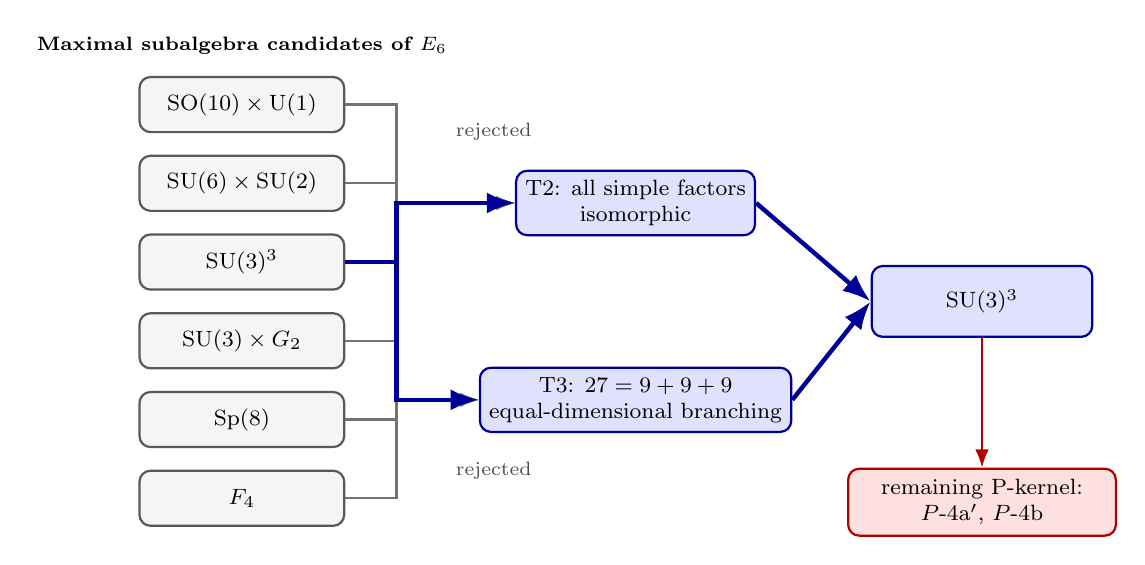
\begin{tikzpicture}[
  >=Latex,
  font=\footnotesize,
  x=1cm,y=1cm,
  cand/.style={draw, rounded corners, thick, align=center,
    minimum width=2.6cm, minimum height=7mm, fill=black!4, draw=black!65},
  filt/.style={draw, rounded corners, thick, align=center,
    minimum width=2.9cm, minimum height=8mm, fill=blue!12, draw=blue!60!black},
  surv/.style={draw, rounded corners, thick, align=center,
    minimum width=2.8cm, minimum height=9mm, fill=blue!12, draw=blue!60!black},
  pbox/.style={draw, rounded corners, thick, align=center,
    minimum width=3.4cm, minimum height=8.5mm, fill=red!12, draw=red!70!black},
  note/.style={font=\scriptsize, align=center}
]

% left column: candidates
\node[cand] (c1) at (0,2.5) {$\SO(10)\times \U(1)$};
\node[cand] (c2) at (0,1.5) {$\SU(6)\times \SU(2)$};
\node[cand] (c3) at (0,0.5) {$\SU(3)^3$};
\node[cand] (c4) at (0,-0.5) {$\SU(3)\times G_2$};
\node[cand] (c5) at (0,-1.5) {$\Sp(8)$};
\node[cand] (c6) at (0,-2.5) {$F_4$};

\node[note] at (0,3.25) {\textbf{Maximal subalgebra candidates of $E_6$}};

% middle filters
\node[filt] (t2) at (5,1.25) {T2: all simple factors\\isomorphic};
\node[filt] (t3) at (5,-1.25) {T3: $27=9+9+9$\\equal-dimensional branching};

% right survivor
\node[surv] (s1) at (9.4,0.0) {$\SU(3)^3$};

% arrows from candidates to filters
\foreach \src in {c1,c2,c3,c4,c5,c6} {
  \draw[->, thick, black!55] (\src.east) -- ++(0.65,0) |- (t2.west);
  \draw[->, thick, black!55] (\src.east) -- ++(0.65,0) |- (t3.west);
}

% highlight surviving path
\draw[->, ultra thick, blue!60!black] (c3.east) -- ++(0.65,0) |- (t2.west);
\draw[->, ultra thick, blue!60!black] (c3.east) -- ++(0.65,0) |- (t3.west);
\draw[->, ultra thick, blue!60!black] (t2.east) -- (s1.west);
\draw[->, ultra thick, blue!60!black] (t3.east) -- (s1.west);

% rejected labels
\node[note, text=black!70] at (3.2,2.15) {rejected};
\node[note, text=black!70] at (3.2,-2.15) {rejected};

% bottom P-kernel
\node[pbox] (pk) at (9.4,-2.55) {remaining P-kernel:\\$P$-4a$'$, $P$-4b};
\draw[->, thick, red!70!black] (s1.south) -- (pk.north);

\end{tikzpicture}
\caption{Candidate-space filtering for trinification inside $E_6$. Among the
six maximal subalgebra candidates, the independent criteria T2 (all simple
factors isomorphic) and T3 (equal-dimensional branching of the 27) both select
$\SU(3)^3$ uniquely. The residual physical arbitrariness is localized at
$P$-4a$'$ and $P$-4b.}
\label{fig:trinification_selection}
\end{figure}

The content of P4a belongs entirely to the M~layer.  Dynkin's classification,
the structural properties of each candidate, and the uniqueness under T2/T3
are all closed by finite enumeration + \texttt{decide}.

\noindent\textit{Lean verification:}
\texttt{M62\_equal\_factor\_selection},
\texttt{M63\_equal\_dim\_branching},
\texttt{three\_factors\_unique} (E6Trinification.lean).


\subsection{Supplemental consistency check}\label{sec:consistency}

The conditional uniqueness of $\SU(3)^3$ is established by M62/M63.  In this
section, a three-axis consistency check based on M-layer theorems is recorded
as a supplement.  The scoring is not a substitute for the uniqueness theorem in
\S\ref{sec:P4a}, but rather an auxiliary means of confirming the physical
differences among the six candidates.

Each axis is based on existing M-layer theorems.  Family consistency (axis~I)
evaluates the correspondence between the outer $(27,3)$ family-triplet
structure (M49) and the inner 27-branching structure.  CP consistency (axis~II)
evaluates whether the unique CP source $\arg(\lambda_3)$ (M52) is cyclically
distributed on the $d_{ijk}$ tensor blocks.  Democracy consistency (axis~III)
corresponds to the degree to which the T2 condition of M62 holds.  The results
are shown in Table~\ref{tab:scoring}.

\begin{table}[htb]
\centering
\caption{Three-axis consistency scoring for $E_6$ maximal
  subalgebras.}\label{tab:scoring}
\begin{tabular}{lcccc}
\toprule
Candidate $H$ & Axis I & Axis II & Axis III & Total \\
\midrule
$\SU(3)^3$ & 3 & 3 & 3 & 9/9 \\
$\SO(10) \times \U(1)$ & 2 & 1 & 1 & 4/9 \\
$\SU(6) \times \SU(2)$ & 1 & 1 & 1 & 3/9 \\
$\SU(3) \times G_2$ & 0 & 0 & 1 & 1/9 \\
$\Sp(8)$ & 0 & 0 & 0 & 0/9 \\
$F_4$ & 0 & 0 & 0 & 0/9 \\
\bottomrule
\end{tabular}
\end{table}

$\SU(3)^3$ is the only candidate that scores the maximum on all three axes,
while the other five score 0 or 1 on at least one axis.  This structure is
robust in the sense of Pareto optimality; $\SU(3)^3$ is no worse than any
other candidate on all axes and strictly better on at least one.

This robustness limits the P-layer content of P-4a$'$.  P-4a$'$ does not
assert the conclusion ``$\SU(3)^3$ is chosen'' (which is closed in~M as a
conditional consequence of M62/M63), but merely the judgment ``equal-rank
democracy (T2 condition) is adopted as a physical principle.''


\subsection{$Z_3$ cyclic symmetry}\label{sec:Z3}

$\SU(3)^3$ has a cyclic permutation $Z_3$ between its three factors:
\begin{equation}\label{eq:Z3}
  \SU(3)_1 \to \SU(3)_2 \to \SU(3)_3 \to \SU(3)_1.
\end{equation}
This $Z_3$ is realized as part of the outer automorphism group of $E_6$.  The
branching $(3,\bar{3},1) \oplus (1,3,\bar{3}) \oplus (\bar{3},1,3)$ is
cyclically permuted under $Z_3$.  The combined total rank of $\SU(3)^3$ and
$\SU(3)_{\mathrm{family}}$ from M58 is $3 \times 2 + 2 = 8 = \rank(E_8)$,
consuming the rank of $E_8$ without excess.

\noindent\textit{Lean verification:}
\texttt{z3\_is\_cyclic}, \texttt{z3\_has\_no\_fixed\_point},
\texttt{full\_chain\_four\_SU3} (E6Trinification.lean).


\subsection{M/P attribution and the P-nucleus remaining in trinification}\label{sec:P-nucleus}

The core of the structural P remaining in trinification is compressed into two
points: P-4a$'$ and P-4b.  The content of P-4a$'$ is refined from the vague
assertion ``choosing trinification'' to the limited and falsifiable assertion
``adopting the physical principle of equal-rank democracy.''  P-4b remains as
an inevitable physical choice: which of the three cyclically symmetric
$\SU(3)$ factors under $Z_3$ is identified as color.

The fact that P-4a$'$ and P-4b are fundamentally impossible to promote to M is
supported by the following proposition.

\begin{proposition}[M-promotion impossibility]\label{prop:M-impossible}
All six maximal subalgebras of $E_6$ exist as well-defined subalgebras.  Based
solely on their algebraic structure, there is no mathematical reason to
consider any one of them as distinguished from the other five.
\end{proposition}

\begin{proof}
By Dynkin's classification theorem, the six candidates correspond to different
embeddings of $E_6$ into the root system, and all are mathematically valid.
The T2/T3 condition is a well-defined predicate on the candidate space, but the
decision to adopt that predicate as a physical selection criterion is not
contained within the algebraic structure.  Similarly, the three factors of
$\SU(3)^3$ are mathematically equivalent by $Z_3$ cyclic symmetry, and there
is no algebraic reason to distinguish one as color.  Therefore, P-4a$'$ and
P-4b structurally remain in~\layerP.
\end{proof}


%% ====================================================================
%%  §6. Minimal Hypothesis Set and Epistemological Significance
%% ====================================================================
\section{Minimal hypothesis set and epistemological
  significance}\label{sec:Sigmamin}


\subsection{Determining the minimum set of hypotheses}\label{sec:determine}

We systematically examine all 25 P-layer hypotheses accumulated through the
research program (complete list in Appendix~\ref{app:Phypotheses}) and
identify the inevitable hypotheses remaining after pushing M-promotion to its
limits.  The minimal hypothesis set $\Amin$ consists of six hypotheses:
\begin{equation}\label{eq:Sigmamin}
  \boxed{\Amin = \bigl\{E_{1a},\; E_{1b},\; E_2,\; E_3,\;
    \text{P-4a}',\; \text{P-4b}\bigr\}.}
\end{equation}

These six hypotheses divide into two groups by their role in the pathway.

\paragraph{Core pathway hypotheses ($A_5 \to E_6 \times A_2 \to \SU(3)^3$):}

\begin{table}[htb]
\centering
\caption{Core pathway hypotheses.}\label{tab:core-hyp}
\begin{tabular}{llll}
\toprule
Hypothesis & Layer & Content & Role \\
\midrule
$E_{1a}$ & \layerE & Spatial dimension $n = 3$ & Step 0--1: $\SO(3) \to A_5$ \\
$E_{1b}$ & \layerE & $\Ngen = 3$ & Step 4--5: C3 for M58 \\
P-4a$'$ & \layerP & Equal-rank democracy & Step 7: $E_6 \to \SU(3)^3$ \\
\bottomrule
\end{tabular}
\end{table}

\paragraph{SM identification hypotheses ($\SU(3)^3 \to \text{SM}$):}

\begin{table}[htb]
\centering
\caption{SM identification hypotheses.}\label{tab:SM-hyp}
\begin{tabular}{llll}
\toprule
Hypothesis & Layer & Content & Role \\
\midrule
$E_2$ & \layerE & Strong force is non-abelian & Step 8: SM identification \\
$E_3$ & \layerE & Asymptotic freedom & Step 8: SM identification \\
P-4b & \layerP & Color identification & Step 8: $\SU(3)^3 \to \text{SM}$ \\
\bottomrule
\end{tabular}
\end{table}


\subsection{Demonstration of completeness}\label{sec:completeness}

By combining the six hypotheses of $\Amin$ with the M-layer theorems, all
steps in the path are uniquely determined; see Table~\ref{tab:completeness}.

\begin{table}[htb]
\centering
\caption{Completeness of the pathway.}\label{tab:completeness}
\begin{tabular}{llll}
\toprule
Step & Input & M-layer theorem & Output \\
\midrule
$0 \to 1$ & $E_{1a}$ ($n = 3$) & Klein~\cite{Klein1884} & Finite subgroups of $\SO(3)$ \\
$1 \to 2$ & $E_{1a}$ + Born law~\cite{Paper1} & M01--M29 & Uniqueness of $A_5$ \\
$2 \to 3$ & --- & Schur multiplier & $2I$ (double cover) \\
$3 \to 4$ & --- & McKay~\cite{McKay1980} & $\Ehat_8$ \\
$4 \to 5$ & $E_{1b}$ ($\Ngen = 3$) & M58 & $E_6 \times A_2$ unique \\
$5 \to 6$ & --- & M49--M57 & Family $= \rho_3'$, CP structure \\
$6 \to 7$ & P-4a$'$ & M62/M63 & $\SU(3)^3$ unique \\
$7 \to 8$ & P-4b + $E_2$ + $E_3$ & SM identification & SM \\
\bottomrule
\end{tabular}
\end{table}

The P-layer hypothesis is not used in Steps~2--4 and 5--6.

The ``Born law'' in Step~$1 \to 2$ refers to the main theorem of
Paper~I~\cite{Paper1}.  Paper~I shows that when the Born probability law
$P(i) = n_i^2/|G|$ (where $n_i$ is the dimension of the irreducible
representation) is defined on a finite subgroup $G$ of $\SO(3)$, the group $G$
must be non-solvable for this distribution to differ from the uniform
distribution.  Since the only non-solvable finite subgroup of $\SO(3)$ under
$n = 3$ is $A_5$ (Klein~\cite{Klein1884}), $A_5$ can be uniquely derived from the
non-triviality of the Born law and $n = 3$.  This process is verified as
M01--M29 in Lean.


\subsection{Demonstration of irreducibility}\label{sec:irreducibility}

We examine the consequences of removing any one hypothesis from $\Amin$ and
show that the unique determination of the path is broken in each case.

\emph{If $E_{1a}$ is removed:} $\SO(3)$ is not determined.  For $n \neq 3$,
the Klein classification is qualitatively different (no non-solvable group for
$n = 2$, no exceptional finite subgroup corresponding to $A_5$ for $n \geq 5$).
The entire path collapses.

\emph{If $E_{1b}$ is removed:} The C3 condition (family dimension~$= 3$) for
M58 becomes undefined.  For $\Ngen \neq 3$, the $E_8$ maximal subalgebra
selection changes ($\Ngen = 2$ leaves $E_7 \times A_1$ as a candidate;
$\Ngen = 5$ makes $A_4 \times A_4$ a candidate).  The uniqueness of $E_6
\times A_2$ is broken.

\emph{If $E_2$ is removed:} The three factors of $\SU(3)^3$ are algebraically
equivalent under $Z_3$ cyclic symmetry, but in SM, one exhibits confinement
as color.  This asymmetric physical role cannot be determined without~$E_2$.

\emph{If $E_3$ is removed:} Asymptotic freedom is independent of
non-abelianity~($E_2$) and is an empirical fact depending on the actual number
of flavors.  Removing $E_3$ makes it impossible to verify the consistency of
coupling running in the trinification~$\to$~SM connection.

\emph{If \textup{P-4a$'$} is removed:} It becomes impossible to uniquely
select $\SU(3)^3$ from the 6 maximal subalgebras of $E_6$.  At least 3
candidates remain: $\SO(10) \times \U(1)$, $\SU(6) \times \SU(2)$, and
$\SU(3)^3$.

\emph{If \textup{P-4b} is removed:} Even after $\SU(3)^3$ is selected, the
physical roles of the three factors remain undetermined.  Due to $Z_3$ cyclic
symmetry, it is not possible to determine which factor is $\SU(3)_C$ from
algebraic means.

In all cases, path uniqueness is broken; therefore irreducibility is satisfied.


\subsection{Previously M-promoted hypotheses}\label{sec:promoted}

As the research program progressed, several hypotheses initially belonging to
layer~P were promoted to layer~M.  Since these have been established as
theorems, they are no longer hypotheses and are not included in~$\Amin$.

\begin{table}[htb]
\centering
\caption{P-layer hypotheses promoted to M-layer.}\label{tab:promoted}
\begin{tabular}{lll}
\toprule
Old P hypothesis & M-layer theorem & Key to promotion \\
\midrule
P-2b ($A_5$ uniqueness) & Klein~\cite{Klein1884} + M01--M29 &
  $n=3$ + non-solvability \\
P-3c ($E_8 \to E_6 \times A_2$) & M58 (\S\ref{sec:M58}) &
  C1+C2+C3 finite enumeration \\
P-3d ($\SU(3)_{\mathrm{fam}} = \rho_3'$) & M49 (\S\ref{sec:M49}) &
  Parity + node~7 removal \\
P-5b (CP $= \arg(\lambda_3)$) & M52 (\S\ref{sec:M52}) &
  Cubic invariant uniqueness \\
\bottomrule
\end{tabular}
\end{table}


\subsection{Distribution and structural significance of P}\label{sec:distribution}

The distribution of the six $\Amin$ hypotheses along the path shows a clear
pattern:
\begin{equation}\label{eq:distribution}
  E_{1a} \longrightarrow
  \underbrace{\text{Steps 1--4}}_{\text{M only}} \longrightarrow
  E_{1b} \longrightarrow
  \underbrace{\text{Steps 5--6}}_{\text{M}} \longrightarrow
  \text{P-4a}' \longrightarrow
  \underbrace{\text{P-4b} + E_2 + E_3}_{\text{SM identification}}.
\end{equation}

The core pathway hypotheses ($E_{1a}$, $E_{1b}$, P-4a$'$) are distributed at
entry, intermediate, and exit points of the pathway, while the SM
identification hypotheses ($E_2$, $E_3$, P-4b) are concentrated in the final
step.  Crucially, the core interval---Steps~1--4 ($A_5 \to 2I \to \Ehat_8$)
and Steps~5--6 (family/CP structure)---is complete in the M~layer without
P-layer intervention.

Note that $\Amin$ is a list of hypotheses \emph{within} the path and does not
include the framework selection $\mathrm{FA}_1$ (\S\ref{sec:mckay}).
$\mathrm{FA}_1$ is not an individual bridge hypothesis but a framework
hypothesis for the entire program, consisting of two components:
$\mathrm{FA}_{1a}$~(canonical lift) and $\mathrm{FA}_{1b}$~(physical
adoption); see~\S\ref{sec:mckay} for the detailed decomposition, the
non-arbitrariness argument, and the counterfactual analysis
(Table~\ref{tab:FA1-counterfactual}).
Therefore, the overall assumption structure of this paper is:
\begin{equation}\label{eq:total-structure}
  \underbrace{\mathrm{FA}_1
    = \mathrm{FA}_{1a} + \mathrm{FA}_{1b}}_{\text{Framework}}
  \;+\;
  \underbrace{\Amin = \{E_{1a}, E_{1b}, E_2, E_3,
    \text{P-4a}', \text{P-4b}\}}_{\text{6 hypotheses within the path}}.
\end{equation}

By explicitly stating this structure---and by decomposing $\mathrm{FA}_1$
into a mathematically motivated component ($\mathrm{FA}_{1a}$) and a genuine
physical commitment ($\mathrm{FA}_{1b}$)---we prevent the criticism of ``not
counting the heaviest assumptions.''


\subsection{Transparency of hypotheses}\label{sec:transparency}

The methodological feature of this program lies not in the total number of
assumptions, but in the consistent traceability of which claims are
mathematical consequences, which are physical hypotheses, and which are
citations of observed facts.  The important point is not to compete on the
number of assumptions, but to clearly indicate where arbitrariness remains in
the theory.


\subsection{Falsifiability of P-4a$'$ and P-4b}\label{sec:falsifiability}

In this paper, only P-4a$'$ and P-4b remain in the P~layer.  Future
observations and model comparisons will focus on these two hypotheses.

If P-4a$'$ is rejected, the conditional uniqueness under M62/M63 itself is not
broken; rather, the reason for physically adopting $\SU(3)^3$ is lost.  Other
$E_6$ maximal subalgebra candidates such as $\SO(10) \times \U(1)$ and $\SU(6)
\times \SU(2)$ would be reintroduced as physical candidates.

Similarly, if P-4b is negated, it is not that the algebraic structure
$\SU(3)^3$ itself is broken, but rather that the assignment of physical roles
to its three factors was incorrect.  Phenomena specific to trinification, such
as decay modes sensitive to color assignment and exotic states, serve as direct
tests.

The most robust quantitative test is the proton decay branching-ratio
pattern.  The $Z_3$ cyclic symmetry of $\SU(3)^3$ (M62, Lean verified:
\texttt{z3\_is\_cyclic}, \texttt{z3\_has\_no\_fixed\_point}) equalizes the
three inter-sector gauge couplings at the trinification scale $M_{\mathrm{tri}}$.
In dimension-6 gauge-boson-mediated decay, the ratio
\begin{equation}\label{eq:RpiK}
  R_{\pi/K}
  \;=\;
  \frac{\Gamma(p \to e^+ \pi^0)}
       {\Gamma(p \to \bar{\nu}\, K^+)}
\end{equation}
factorizes as
$R_{\pi/K} = (\text{flavor ratio})
  \times (W_\pi / W_K)^2
  \times (\text{phase space ratio})$.
In minimal $\SU(5)$, the flavor factor is $|V_{ud}/V_{us}|^2 \approx 19$
(CKM suppression of the $\Delta S = 1$ channel), giving $R_{\pi/K} \approx 43$.
In $\SU(3)^3$ trinification, $Z_3$ democracy sets the flavor ratio to unity
at $M_{\mathrm{tri}}$; Yukawa running corrections are negligible
($\delta f/f \sim y_s^2 \ln(M_{\mathrm{tri}}/m_p)/(16\pi^2) \ll 1$).
Including $\sim 20\%$ lattice uncertainty on the hadronic matrix elements
$W_{\pi,K}$, one obtains
\begin{equation}\label{eq:RpiK-value}
  R_{\pi/K}^{\,\SU(3)^3} \;\in\; [1, 5],
  \qquad
  R_{\pi/K}^{\,\SU(5)} \approx 43.
\end{equation}
The factor-of-$\sim 19$ separation is structural: it originates entirely from
CKM~vs.\ $Z_3$-democracy and does \emph{not} depend on $M_{\mathrm{tri}}$
(which cancels in the ratio) or on threshold corrections.
Table~\ref{tab:proton_decay} summarizes the comparison.

\begin{table}[t]
\centering
\caption{Proton decay branching-ratio discriminants.
$R_{\pi/K}$ is defined in Eq.~\eqref{eq:RpiK}.
The $\SU(3)^3$ column follows from $Z_3$ cyclic symmetry
(M62, Lean verified) and is independent of $M_{\mathrm{tri}}$.
Hadronic matrix elements carry $\sim 20\%$ lattice uncertainty.}
\label{tab:proton_decay}
\begin{tabular}{lccc}
\toprule
Observable & $\SU(5)$ & SO(10) (SUSY) & $\SU(3)^3$ + $A_5$ \\
\midrule
Dominant mode & $p \to e^+\pi^0$ & $p \to \bar\nu K^+$ & $p \to e^+\pi^0$ \\
$R_{\pi/K}$ & $\approx 43$ & $\ll 1$ & $1$--$5$ \\[2pt]
$R_{\ell/\nu}$ & $> 1$ & $< 1$ & $\approx 1$ \\
Flavor origin & CKM & CKM + seesaw & $A_5$ CG ($\rho_3'$) \\
$M_{\mathrm{GUT}}$-indep.? & no & no & yes (ratio) \\
P-4b test & --- & --- & $\checkmark$ \\
\bottomrule
\end{tabular}
\end{table}

The ratio $R_{\ell/\nu} = \Gamma(p \to \ell^+ + \text{meson})
/ \Gamma(p \to \bar\nu + \text{meson})$ provides a second discriminant.
The $Z_3$ symmetry relates the $(Q \to L)$ and $(Q \to \bar{Q})$
inter-sector transitions symmetrically, yielding $R_{\ell/\nu} \approx 1$,
in contrast to SUSY~$\SO(10)$ where dimension-5 operators give
$R_{\ell/\nu} < 1$.

For P-4b, different assignments of $\SU(3)_C$ among the three
$Z_3$-equivalent factors lead to different branching-ratio patterns,
making P-4b an experimentally falsifiable hypothesis.
These predictions can be tested at Hyper-Kamiokande and DUNE.


%% ====================================================================
%%  §7. Comparison with other theories and future prospects
%% ====================================================================
\section{Comparison with other theories and future
  prospects}\label{sec:comparison}


\subsection{Relationship with existing discrete symmetry models}\label{sec:discrete}

Numerous models based on discrete flavor symmetry have been proposed (see
reviews~\cite{Feruglio2015,KingLuhn2013}).  $A_4$ (order~12) is widely used to
explain the tri-bimaximal mixing pattern~\cite{Ma2001,AltarelliFeruglio2006},
and $S_4$ (order~24) has been applied to atmospheric mixing angle
maximality~\cite{Lam2008}.  $\Delta(27)$ (order~27) contains a complex
structure for CP violation~\cite{LuhnNasriRamond2007}.

The $A_5$ (order~60) adopted by this program is fundamentally different in the
following respects.

First, $A_5$ is uniquely characterized as a non-solvable finite subgroup of
$\SO(3)$ (Paper~I~\cite{Paper1} main theorem).  $A_4$ and $S_4$ are both
solvable and lack a comparable uniqueness justification.

Second, the fact that all irreducible representations of $A_5$ are real
type~(M50) allows a clear attribution of the CP phase origin to structures
outside $A_5$.  For $A_4$ and $\Delta(27)$, complex representations exist, and
the origin of CP is intertwined with the internal structure of the group,
making M/P separation difficult.

Third, the connection to $E_8$ through the McKay correspondence is unique to
$A_5$.  $A_4$, $S_4$, and $\Delta(27)$ are finite subgroups of $\SO(3)$, but
the McKay correspondence holds for finite subgroups of $\SU(2)$---that is,
double covering groups.  The double cover $2I$ of $A_5$ gives an $E_8$-type
McKay graph, but the double covers $2T$ of $A_4$ ($E_6$~type) and $2O$ of
$S_4$ ($E_7$~type) do not reach $E_8$.

On the other hand, this program has significant limitations that need explicit
statement.  First, individual fermion masses and mixing angles are not yet
predicted; these require completion of the VEV analysis for the 19-parameter
$A_5$-invariant potential, which is ongoing.  However, the framework does yield
structural predictions at the present stage: the proton decay ratio
$R_{\pi/K} \in [1,5]$, qualitatively distinct from
$R_{\pi/K}^{\,\SU(5)} \approx 43$
(\S\ref{sec:falsifiability}, Table~\ref{tab:proton_decay}),
and the structural necessity of $\theta_{13} \neq 0$.
On the latter point, $A_4$ models predicted $\theta_{13} = 0$ under
tri-bimaximal mixing and were falsified by Daya Bay (2012);
in the $A_5$ framework, $\rho_3$ and $\rho_3'$ are non-isomorphic
Galois conjugates (M29), and the Channel~III mixing matrix
($\rho_3 \otimes \rho_3' \otimes \rho_4$, M57) generically has a non-vanishing
1--3 component, making $\theta_{13} \neq 0$ a structural consequence
rather than a parameter adjustment.
Second, the rationale for physically adopting the McKay path
($\mathrm{FA}_1$) is a framework choice fundamentally different from
``justification by fitting.''


\subsection{Relationship with $E_8$ unified theory}\label{sec:E8unified}

The approach of using $E_8$ as a unifying group has been widely studied in the
context of heterotic string theory~\cite{GrossHarveyMartinecRohm1985}.  In
this program, $E_8$ is obtained independently of string compactification, from
the McKay correspondence.  The idea of applying the algebraic structure of
$E_8$ to family unification is also seen in Ramond~\cite{Ramond2001}, but this
program starts from the McKay correspondence.

The Griess--Ryba~\cite{GriessRyba1999} classification of finite group
embeddings into $E_8$ refines the positioning of $2I$ within $E_8$.  The
$\mathrm{G1}'$~programme of this program aims to concretize the connection
between McKay and Lie algebraic paths by computing the structure of
$C_{E_8}(2I)$ using GAP.

Dechant's~\cite{Dechant2013} Clifford algebraic approach illuminates the
icosahedron--$E_8$ relationship from a different perspective.  Its relation to
this program is formally recorded in G1SelCore.lean as
\texttt{dechant\_not\_SU3\_class}.


\subsection{Future outlook}\label{sec:outlook}

\paragraph{Short term.}
(i)~Paper~V (CP violation): based on the CP structure of M50--M57 (\S\ref{sec:CP}),
quantitative prediction of $\delta_{\mathrm{CP}}$ via swap-odd structures and
VEV mechanics.  The scope of M52 is limited to renormalizable theory; a
systematic analysis of higher-dimensional effective operators is also included.
(ii)~Numerical refinement of $R_{\pi/K}$: the structural prediction
$R_{\pi/K} \in [1,5]$ (\S\ref{sec:falsifiability}) will be sharpened
by incorporating one-loop RG running from $M_{\mathrm{tri}}$ to $m_p$
and the $A_5$ Clebsch--Gordan corrections from the $\rho_3'$ family
structure (M49).  A preliminary analysis using one-loop SM running
gives $\alpha_2^{-1}(M_{\mathrm{tri}}) = \alpha_3^{-1}(M_{\mathrm{tri}})$
at $\log_{10}(M_{\mathrm{tri}}/\mathrm{GeV}) \approx 17.0$, with
threshold corrections admitting a window
$\log_{10}(M_{\mathrm{tri}}/\mathrm{GeV}) \in [15, 19]$.
(iii)~$A_5$-specific corrections to $R_{e/\mu} = \Gamma(p \to e^+\pi^0)
/ \Gamma(p \to \mu^+\pi^0)$, arising from the $\rho_3'$ tensor product
decomposition $\rho_3' \otimes \rho_3' = \rho_1 \oplus \rho_3 \oplus \rho_5$
(M01, Lean verified), will be computed after Phase~3 (Channel~III
Clebsch--Gordan completion).

\paragraph{Mid-term.}
(iv)~$\mathrm{G1}'$~programme: computing $C_{E_8}(2I)$ in GAP to directly
connect the McKay path ($A_5 \to 2I \to E_8$) and the Dynkin--Lie path ($E_8
\to E_6 \times A_2 \to \SU(3)^3$), potentially elevating ``uniqueness as
selection'' (M58) to ``uniqueness as embedding.''
(v)~Gauge coupling unification: extending the preliminary one-loop analysis
of~(ii) to two-loop running with threshold corrections, and comparing the
$\SU(3)^3$ unification window with those of $\SO(10) \times \U(1)$ and
$\SU(6) \times \SU(2)$ to further constrain P-4a$'$.

\paragraph{Long term.}
(vi)~Origin of the Lorentz group and gravity: deriving spacetime symmetries
from the same algebraic framework; null-count kernels and the edge-strain
variational principle are candidate approaches.
(vii)~Complete description of the mass hierarchy: the $A_5$ flavor structure
gives a mass/mixing Galois splitting~(M57), but specific fermion masses depend
on VEV dynamics.  Phase structure analysis of the 19-parameter $A_5$-invariant
potential is underway.


%% ====================================================================
%%  §8. Conclusion
%% ====================================================================
\section{Conclusion}\label{sec:conclusion}

In this paper, the entire pathway $A_5 \to 2I \to \Ehat_8 \to E_6 \times A_2
\to \SU(3)^3 \to \text{SM}$ was dissected under epistemological three-layer
separation (M/P/E), and the following two main results were established.

\paragraph{Main result~1 (rigidity).}
Under the framework hypothesis $\mathrm{FA}_1$, the core pathway $A_5 \to 2I
\to \Ehat_8 \to E_6 \times A_2$ is uniquely fixed in layer~M with
$E_{1a}$~($n=3$) and $E_{1b}$~($\Ngen = 3$) as the sole external inputs.
More than 60 named theorems (M01--M63 and supporting results), including
M49--M63, have been formally verified by
Lean~4 with \texttt{sorry\,=\,0} and \texttt{axiom\,=\,0}; the precise scope
of what the type-checker guarantees is detailed in~\S\ref{subsec:lean-scope}.
Note that M52
(uniqueness of CP source) holds only for the renormalizable sector; additional
CP sources from effective operators of $\dim \geq 5$ fall within the scope of
Paper~V.

\paragraph{Main result~2 (localization).}
$\Amin = \{E_{1a}, E_{1b}, E_2, E_3, \text{P-4a}', \text{P-4b}\}$ is
complete and irreducible.  The structural degrees of freedom belonging to the
P-layer are localized at two points: P-4a$'$ and P-4b.

The epistemological significance of these results can be summarized as follows.

First, this paper establishes the precise identification of the M/P boundary.
This boundary accurately identifies areas that need improvement---for example,
the M-promotion of P-4a$'$ or the direct McKay--Lie pathway connection by the
$\mathrm{G1}'$~programme.

Second, all M-layer theorems have been mechanically verified using a Lean~4
type checker, and these mathematical consequences are irrevocable.  Only the
two P-layer hypotheses (P-4a$'$ and P-4b) and the physical-adoption component
$\mathrm{FA}_{1b}$ of the framework hypothesis may be modified by future
observations or theoretical developments.  If $\mathrm{FA}_1$ is rejected,
the M-layer theorems remain valid as pure mathematics; only their physical
interpretation is withdrawn (\S\ref{sec:mckay},
Table~\ref{tab:FA1-counterfactual}).

Third, the concentration of falsifiability on P-4a$'$ and P-4b limits the
focus of experimental verification (\S\ref{sec:falsifiability}).  The $Z_3$
cyclic symmetry of $\SU(3)^3$ (M62) yields a concrete, $M_{\mathrm{tri}}$-independent
discriminant: $R_{\pi/K} \in [1,5]$, separated by a factor of $\sim 19$ from
the minimal $\SU(5)$ prediction (Table~\ref{tab:proton_decay}).  If
experiments reject P-4a$'$, it is not the rigidity of the core pathway that
collapses, but only the physical adoption of trinification, and the candidate
space of $E_6$ (M62/M63) is reopened.

Finally, the methodology of this paper---attributing all claims to M/P/E and
machine-verifying the M~layer---is not specific to the $A_5$ program but is a
general framework applicable to any BSM physics theory.  Maintaining constant
traceability of the boundary between mathematical consequences and physical
hypotheses, and supporting this with formal verification, proposes a new
standard for assumption management in theoretical physics.

%%============================================================
%% Acknowledgments + Declarations (Springer Nature mandatory)
%% ============================================================
\backmatter

\bmhead{Acknowledgments}

The formal verification in this paper is based on the Lean~4
theorem prover~\cite{Lean4} and the Mathlib mathematical
library~\cite{Mathlib}.
The author thanks the developer communities of both projects.

\bmhead{Statements and Declarations}

\paragraph{Funding.}
This research received no external funding.

\paragraph{Competing interests.}
The author declares no competing interests.

\paragraph{Ethics approval and consent to participate.}
Not applicable.

\paragraph{Consent for publication.}
Not applicable.

\paragraph{Data availability.}
No experimental data were generated or analysed in this study.
All numerical values of physical constants are taken from published
sources cited in the bibliography.
The Lean~4 source code and numerical computations supporting the
results are publicly available at
\url{https://github.com/nuu/A5_SM_Pathway}
and permanently archived at Zenodo
(\url{https://doi.org/10.5281/zenodo.18801089})
under the Apache License~2.0.

\paragraph{Materials availability.}
Not applicable.

\paragraph{Code availability.}
The complete Lean~4 source code for the formal verification
(sorry\,$=$\,0, axiom\,$=$\,0) and the theorem--identifier
correspondence table are publicly available at
\url{https://github.com/nuu/A5_SM_Pathway}
and permanently archived at Zenodo
(\url{https://doi.org/10.5281/zenodo.18801089})
under the Apache License 2.0.
The repository includes all files necessary to reproduce
the verification: \texttt{lakefile.lean}, Mathlib dependency
specifications, and per-section Lean source files
(\texttt{Section1\_Introduction.lean} through
\texttt{Section8\_Conclusion.lean} and auxiliary modules).

\paragraph{Author contribution.}
M.~Numagaki is the sole author and is responsible for the
conception of the theoretical framework,
all mathematical proofs and their Lean~4 formalization,
the numerical analysis, and the writing of the manuscript.

\paragraph{Use of AI-assisted tools.}
Use of Generative AI and AI-assisted technologies in the writing process
During the preparation of this work the author used ChatGPT in order to improve the readability and language of the manuscript. After using this tool/service, the author reviewed and edited the content as needed and takes full responsibility for the content of the publication.

%% ====================================================================
%%  Appendix A: Lean 4 Verification System
%% ====================================================================
\begin{appendices}

\section{Lean~4 verification system}\label{app:lean}

\subsection{Project overview}

The M-layer theorems in this research program are implemented as a formal proof
project called ``A5\_SM\_Pathway'' using Lean~4 + Mathlib.  While there are
precedents for large-scale formal verification in mathematics (such as the
Kepler conjecture~\cite{Hales2017}), to the best of the author's knowledge,
there are no precedents for applying formal verification of this scale to the
theoretical structure of elementary particle physics.

\begin{table}[htb]
\centering
\caption{A5\_SM\_Pathway project statistics.}\label{tab:project-stats}
\begin{tabular}{ll}
\toprule
Item & Value \\
\midrule
Project name & A5\_SM\_Pathway \\
Number of files & $\sim$45 \\
Total lines & $\sim$10\,800 \\
\texttt{sorry} & 0 \\
\texttt{axiom} & 0 \\
Main theorems & 60+ (named M01--M63) \\
Total Lean \texttt{theorem} declarations & $\sim$200 (incl.\ supporting lemmas) \\
Build system & \texttt{lake build} \\
Zenodo DOI & 10.5281/zenodo.18801089 \\
GitHub & github.com/nuu/A5\_SM\_Pathway \\
\bottomrule
\end{tabular}
\end{table}

\texttt{sorry\,=\,0} means all theorems have been proven with no unproven
holes.  \texttt{axiom\,=\,0} means no additional axioms beyond the standard
Lean/Mathlib axioms have been used.


\subsection{Scope and limitations of formal verification}
\label{subsec:lean-scope}

It is essential to state precisely what the Lean type-checker does and does not
guarantee.  Table~\ref{tab:lean-scope} summarizes the boundary.

\begin{table}[htb]
\centering
\caption{Scope of the Lean~4 verification.}\label{tab:lean-scope}
\begin{tabular}{p{0.46\textwidth}p{0.46\textwidth}}
\toprule
\textbf{Verified by the type-checker} & \textbf{Not verified by the type-checker} \\
\midrule
Given the hand-encoded finite data (character tables, Dynkin diagram
adjacencies, Cartan matrix entries, maximal-subalgebra lists),
all logical consequences drawn from those data are
machine-checked with no gaps.
&
The correctness of the hand-encoded data itself.
For example, the values
$\chi_{\rho_3}(C_5^+) = \varphi = (1+\sqrt{5})/2$
and
$\mathtt{nodeRemovalResult\;.n7} = [\mathtt{.E6},\;\mathtt{.A\;2}]$
are typed by the author.  If an entry were mis-transcribed, Lean
would still accept the proofs.
\\[4pt]
Exhaustive case-split over all elements of a finite type
(\texttt{decide}/\texttt{native\_decide}), ensuring no case is
missed.
&
The identification of the finite type with its mathematical
counterpart (e.g.\ that the 8-element type \texttt{E8MaxSub}
faithfully represents Dynkin's classification of $E_8$ maximal
subalgebras).
\\[4pt]
Arithmetic in $\mathbb{Q}(\sqrt{5})$ (the ring \texttt{QSqrt5})
and $\mathbb{Z}$-matrix algebra (\texttt{Mat8}).
&
The McKay correspondence theorem itself, the Dynkin classification
theorem, and the Griess--Ryba classification.  These are cited as
established mathematical results and encoded as data, not proved
from first principles in Lean.
\\
\bottomrule
\end{tabular}
\end{table}

\paragraph{Mitigation.}
The risk of data-entry error is mitigated by three independent measures.
(1)~\emph{Internal consistency checks}: Lean verifies $\sum d_i^2 = 60$
(A$_5$ order), $\sum d_i^2 = 120$ (2I order), $\sum\text{marks} = 30$
(Coxeter number), $\sum\text{branch dims} = 248$, and Cayley--Hamilton for
the $E_8$ Cartan matrix.  A single mis-transcribed entry would generically
violate at least one such check.
(2)~\emph{Dual encoding}: the A$_5$ character table is independently encoded
in both \texttt{FlavorCharTable.lean} and \texttt{A5CP.lean}, with no import
dependency between them; agreement serves as a cross-check.
(3)~\emph{Independent GAP/Python verification}: every hand-encoded datum is
also verified by GAP~4.15.1 and/or Python scripts (Appendix~\ref{app:gap}),
providing a third implementation on a different code base.

\paragraph{What ``63+ theorems'' means.}
The project contains approximately 200 Lean \texttt{theorem} declarations in
total, including supporting lemmas, \texttt{@[simp]} rewriting rules, and
structural bookkeeping (e.g.\ \texttt{file\_integrity :\ True := trivial}).
The ``60+ named theorems'' cited in this paper refer to the M01--M63
series and their direct corollaries---those with substantive mathematical
content corresponding to numbered results in the text.  Three declarations
(\texttt{M57\_rho4\_integer\_char}, \texttt{M57\_rho5\_integer\_char},
\texttt{file\_integrity}) have the trivial statement \texttt{True} and serve
only as registry markers; they are not counted among the substantive
theorems.


\subsection{Main files and correspondence theorems}

\begin{table}[htb]
\centering
\caption{Main Lean files and their theorem coverage.}\label{tab:lean-files}
\begin{tabular}{llrl}
\toprule
File & Main theorems & Lines & Technique \\
\midrule
QSqrt5.lean & $\mathbb{Q}(\sqrt{5})$ construction & $\sim$200 & constructive \\
FlavorCharTable.lean & M01--M03, M11, M28 & $\sim$140 & \texttt{native\_decide} \\
FlavorCore.lean & CG tensor construction & $\sim$100 & constructive \\
FlavorGalois.lean & M07, M19, M29, M30 & $\sim$220 & \texttt{native\_decide} \\
A5CP.lean & M49, M50, M53--M57 & $\sim$350 & \texttt{decide}/\texttt{native\_decide} \\
E6Complex.lean & M51 (27 complex type) & $\sim$200 & \texttt{decide} \\
E8MaxSub.lean & M58 & $\sim$200 & \texttt{decide} \\
E8BlowUp.lean & M59--M61 & $\sim$350 & \texttt{decide} \\
E8Cartan.lean & Cartan matrix eigenvalues & $\sim$200 & \texttt{decide} \\
E6Trinification.lean & M62--M63, $Z_3$ structure & $\sim$270 & \texttt{decide} \\
G1SelCore.lean & Consequence layer & $\sim$310 & constructive \\
\bottomrule
\end{tabular}
\end{table}


\subsection{Overview of the verification method}

The three main proof methods used in this project are:

\texttt{decide}: Fully automated proof for decidable predicates.  The truth
value is determined by exhaustive traversal on a finite type.  The main
theorems of E8MaxSub.lean (8 candidates), E8BlowUp.lean (9 nodes),
E6Trinification.lean (6 candidates), and E6Complex.lean (M51) are all closed
by this method.

\texttt{native\_decide}: The native code version of \texttt{decide},
evaluating using compiled code rather than the Lean kernel evaluator.  Used in
character table calculations involving $\mathbb{Q}(\sqrt{5})$ arithmetic, such
as FlavorCharTable.lean and A5CP.lean.

\emph{Constructive proof}: General type-theoretic methods (\texttt{intro},
\texttt{apply}, \texttt{exact}, \texttt{simp}, \texttt{ring}, etc.)\ used in
QSqrt5.lean (field structure of $\mathbb{Q}(\sqrt{5})$) and
AddressPrinciple.lean (Paper~I main theorem).


\subsection{Dependencies}

The dependencies between the main files are:
\begin{verbatim}
QSqrt5.lean
  +-- FlavorCharTable.lean
  |     +-- FlavorGalois.lean (M07, M19, M29, M30)
E6Complex.lean (M51, independent)
  +-- A5CP.lean (M49, M50, M53-M57)
E8MaxSub.lean (M58, independent)
E8BlowUp.lean (M59-M61, independent)
E8Cartan.lean (independent)
E6Trinification.lean (M62-M63, independent)
FlavorCore.lean (independent)
G1SelCore.lean (independent)
\end{verbatim}

A5CP.lean defines the necessary character table data for M49--M57 in a
self-contained manner and has no import relationship with
FlavorCharTable.lean, constituting independent dual validation.
M51, M58, M59--M61, M62--M63, and FlavorCore are all independent files,
structurally guaranteeing the independence of each theorem.


\subsection{Reproduction steps}

\begin{enumerate}
  \item Install Lean~4 and Lake (Lean's build system).
  \item Clone the repository:
    \texttt{git clone https://github.com/nuu/A5\_SM\_Pathway}
  \item Execute \texttt{lake build}.
  \item Type checking of all theorems is complete; confirm no
    \texttt{sorry}/axioms.
\end{enumerate}

The Mathlib version is pinned in \texttt{lakefile.lean}.


%% ====================================================================
%%  Appendix B: GAP Verification Scripts
%% ====================================================================
\section{GAP verification scripts}\label{app:gap}

\subsection{Environment}

\begin{table}[htb]
\centering
\caption{GAP verification environment.}\label{tab:gap-env}
\begin{tabular}{ll}
\toprule
Item & Value \\
\midrule
System & GAP 4.15.1 (Windows) \\
Main package & CTblLib (Character Table Library) \\
Usage & Computational verification of character tables and representations \\
\bottomrule
\end{tabular}
\end{table}

Verification using GAP is a computational method independent of Lean formal
proofs, providing a double guarantee of reliability by verifying the same
theorem with different implementations.


\subsection{Script list}

\begin{table}[htb]
\centering
\caption{GAP/Python verification scripts.}\label{tab:gap-scripts}
\begin{tabular}{llll}
\toprule
Script & Verification & Main output & Result \\
\midrule
M50\_M54\_verify.gap & M50 ($\nu_2$), M54 (initial) &
  FS $= [1,1,1,1,1]$ & PASS \\
M54\_corrected\_v2.gap & M54 (GaloisCyc$(\cdot,2)$) &
  $\sigma$ permutation & PASS \\
M52a\_verify\_v2.gap & M52a ($\Sym^3(27)$ inv.) &
  $\dim \Inv = 1$ & PASS \\
B4\_node\_removal.gap & M59 ($\Ehat_8$ node removal) &
  9 Dynkin types & PASS \\
M58\_verify.py & M58 (selection + 248 branching) &
  Survivor $= [E_6 \times A_2]$ & PASS \\
\bottomrule
\end{tabular}
\end{table}


\subsection{Technical notes}

In the verification of M54, the initial script used
$\mathrm{GaloisCyc}(x, -1)$ (complex conjugate), which could not detect the
Galois automorphism~$\sigma$.  We confirmed that $\mathrm{GaloisCyc}(x, 2)$
--- acting as $\zeta_5 \mapsto \zeta_5^2$ and inducing $\sqrt{5} \mapsto
-\sqrt{5}$ --- is the correct implementation, by applying it to $\sqrt{5} =
\mathrm{E}(5) + \mathrm{E}(5)^4 - \mathrm{E}(5)^2 - \mathrm{E}(5)^3$.

M58\_verify.py is a Python script that includes automatic node removal
determination for affine $\Ehat_8$ (Dynkin type classification by arm length
analysis) and dimensional consistency checks for 248 branching, providing a
third verification method independent of the GAP script.


\subsection{Complementarity with Lean verification}

The three methods---Lean, GAP, and Python---are based on different
implementation foundations and provide independent confirmations.  In
particular, M58 undergoes triple validation using Lean (\texttt{decide}), GAP
(character table + FS indicator), and Python (node removal + dimension check).


%% ====================================================================
%%  Appendix C: Complete list of P-layer hypotheses
%% ====================================================================
\section{Complete list of P-layer hypotheses}\label{app:Phypotheses}

In this research program, 25 numbered P-layer hypotheses have been identified.
In this paper, the former E1 has been separated into $E_{1a}$ (spatial
dimension) and $E_{1b}$ (number of generations).

\subsection{M-promoted (not included in $\Amin$)}

\begin{table}[htb]
\centering
\caption{P-layer hypotheses promoted to M-layer.}\label{tab:C1}
\begin{tabular}{llll}
\toprule
ID & Hypothesis & M-theorem & Lean verified \\
\midrule
P-2a & Non-solvability required & Born law (Paper~I) & $\checkmark$ \\
P-2b & $A_5$ uniqueness & Klein~\cite{Klein1884} + M01--M29 & $\checkmark$ \\
P-3c & $E_8 \to E_6 \times A_2$ & M58 (\S\ref{sec:M58}) & $\checkmark$ \\
P-3d & $\SU(3)_{\mathrm{fam}} = \rho_3'$ & M49 (\S\ref{sec:M49}) &
  $\checkmark$ \\
P-5b & CP $= \arg(\lambda_3)$ & M52 (\S\ref{sec:M52}) & $\checkmark$ \\
P-9b & $\SO(3)$ finite subgroups & Klein~\cite{Klein1884} & --- \\
\bottomrule
\end{tabular}
\end{table}


\subsection{Observational facts (included in $\Amin$)}

\begin{table}[htb]
\centering
\caption{Observational-fact hypotheses in $\Amin$.}\label{tab:C2}
\begin{tabular}{lll}
\toprule
ID & Hypothesis & $\Amin$ name \\
\midrule
P-1a & $n = 3$ + spinors & $E_{1a}$ \\
--- & $\Ngen = 3$ & $E_{1b}$ \\
P-3a & Non-abelian strong force & $E_2$ \\
P-3b & Asymptotic freedom & $E_3$ \\
\bottomrule
\end{tabular}
\end{table}


\subsection{Structural P (included in $\Amin$)}

\begin{table}[htb]
\centering
\caption{Structural P-layer hypotheses in $\Amin$.}\label{tab:C3}
\begin{tabular}{llll}
\toprule
ID & Hypothesis & $\Amin$ name & Rationale \\
\midrule
P-4a$'$ & Equal-rank democracy & P-4a$'$ & Physical adoption of T2 \\
P-4b & Color identification & P-4b & $Z_3$ physical selection \\
\bottomrule
\end{tabular}
\end{table}


\subsection{Outside the scope of Paper~IV}

14 additional hypotheses (P-3e, P-5c, P-6, P-6b--d, P-7a--d, P-8a--c, P-9a)
belong to other papers (Paper~III, Paper~V, $\mathrm{G1}'$~programme) and do
not affect $\Amin$.  See Table~\ref{tab:C4} for the complete list.

\begin{table}[htb]
\centering
\caption{P-layer hypotheses outside the scope of Paper~IV.}\label{tab:C4}
\begin{tabular}{lll}
\toprule
ID & Hypothesis & Affiliation \\
\midrule
P-3e & $E_6$ branch is physical & Paper~IV \S7 \\
P-5c & $\delta_{\mathrm{CP}} \approx 70^\circ$ & Paper~V \\
P-6 & $\tau$-preceding condensation & Paper~III \\
P-6b & $r_c$ is small & Paper~III \\
P-6c & $\xi \approx 0.13$ & Paper~III \\
P-6d & $\theta_{23} \approx 13^\circ$ & Paper~III \\
P-7a & $A_5$ = singularity information source & $\mathrm{G1}'$ \\
P-7b & Area $\approx 1/g^2$ & $\mathrm{G1}'$ \\
P-7c & $\beta^* \leftrightarrow$ K\"ahler & $\mathrm{G1}'$ \\
P-7d & 4.33\,TeV & $\mathrm{G1}'$ \\
P-8a & Cubic Yukawa domination & Paper~III \\
P-8b & Channel~II $=$ residual mass & Paper~III \\
P-8c & Mass hierarchy correspondence & Paper~V \\
P-9a & Identifying ``natural occurrences'' & Whole program \\
\bottomrule
\end{tabular}
\end{table}


\subsection{Aggregation}

\begin{table}[htb]
\centering
\caption{Summary of P-layer hypothesis classification.}\label{tab:C-summary}
\begin{tabular}{lcl}
\toprule
Category & Count & In $\Amin$? \\
\midrule
M-promoted & 6 & No (established as theorems) \\
Observational facts \layerE & 3 & Yes ($E_{1a}$, $E_2$, $E_3$) \\
Structural P & 2 & Yes (P-4a$'$, P-4b) \\
Outside scope & 14 & No (other papers) \\
\midrule
Total (numbered) & 25 & --- \\
Added decomposition & $+1$ & $E_{1b}$ ($\Ngen = 3$) \\
\midrule
\textbf{Total $\Amin$} & \textbf{6} & 4\,\layerE\ $+$ 2\,\layerP \\
\bottomrule
\end{tabular}
\end{table}

The completeness of $\Amin$ is guaranteed by the fact that, excluding the 6
M-promoted and 14 out-of-scope hypotheses from the 25 numbered ones, and
adding $E_{1b}$ (explicitly revealed by the separation of the old~E1), 6
hypotheses (4~\layerE\ $+$ 2~\layerP) cover all steps of the path
(Table~\ref{tab:completeness}).  Irreducibility is guaranteed by the fact that
removing any one of the 6 hypotheses renders the path indeterminate
(\S\ref{sec:irreducibility}).


\end{appendices}

%% ====================================================================
%%  References
%% ====================================================================
\bibliography{refs}

\end{document}
